\documentclass[manuscript,screen,review]{acmart}

\usepackage{graphicx}
\usepackage{hyperref}
\usepackage[utf8]{inputenc}
\usepackage{booktabs}
\usepackage{url}
\usepackage{comment}
\usepackage{microtype}
\usepackage{siunitx}
\usepackage{subcaption}
\sisetup{output-exponent-marker=\ensuremath{\mathrm{e}}}
\usepackage{wrapfig}
\usepackage{tabularx}
\usepackage{ragged2e}


\pdfstringdefDisableCommands{%
  \def\unskip#1{<#1>}%
}

%%
%% \BibTeX command to typeset BibTeX logo in the docs
\AtBeginDocument{%
  \providecommand\BibTeX{{%
    Bib\TeX}}}

%% Rights management information.  This information is sent to you
%% when you complete the rights form.  These commands have SAMPLE
%% values in them; it is your responsibility as an author to replace
%% the commands and values with those provided to you when you
%% complete the rights form.
% \setcopyright{acmcopyright}
% \copyrightyear{2018}
% \acmYear{2018}
% \acmDOI{XXXXXXX.XXXXXXX}

%% These commands are for a PROCEEDINGS abstract or paper.
% \acmConference[Conference acronym 'XX]{Make sure to enter the correct
%   conference title from your rights confirmation email}{June 03--05,
%   2018}{Woodstock, NY}
%%
%%  Uncomment \acmBooktitle if the title of the proceedings is different
%%  from ``Proceedings of ...''!
%%
%%\acmBooktitle{Woodstock '18: ACM Symposium on Neural Gaze Detection,
%%  June 03--05, 2018, Woodstock, NY}
% \acmPrice{15.00}
% \acmISBN{978-1-4503-XXXX-X/18/06}


%%
%% Submission ID.
%% Use this when submitting an article to a sponsored event. You'll
%% receive a unique submission ID from the organizers
%% of the event, and this ID should be used as the parameter to this command.
%%\acmSubmissionID{123-A56-BU3}

\renewcommand\UrlFont{\color{blue}\rmfamily}

%%
%% end of the preamble, start of the body of the document source.
\begin{document}

% Per ACM Computing Surveys Call:

% https://dl.acm.org/journal/csur/author-guidelines

% The ACM Computing Surveys publishes surveys of and tutorials on areas of computing research or practice.
% Long paper (ours)
%   Summarizes and organizes recent research results in a novel way 
%   Integrates and adds understanding to work in the field
%   Assumes a general knowledge of the area
%   Emphasizes 
%     Classification of the existing literature
%     Developing a perspective on the area
%     Evaluating trends
% Length
%   Should normally not exceed 35 pages, including references
%   When justified, additional material may be considered or published in an electronic supplement 
%   You will need to go through the manuscript and indicate which pages will form your 35 pages for publication and which pages are for the electronic supplement
%   Manuscripts of excessive length may be rejected without review
% Use of the ACM Journals/Transactions LaTeX style is encouraged to ensure proper formatting
% A footnote on the first page should acknowledge funding sources and presentations
% Author's current address should be given in a footnote on the first page.
% 


%%
%% The "title" command has an optional parameter,
%% allowing the author to define a "short title" to be used in page headers.
\title{Examining Multimodal Methods for Analyzing Learning and Training Environments: A Systematic Literature Review}

%%
%% The "author" command and its associated commands are used to define
%% the authors and their affiliations.
%% Of note is the shared affiliation of the first two authors, and the
%% "authornote" and "authornotemark" commands
%% used to denote shared contribution to the research.

\author{Anonymous Author 1}
\email{anonymous@anonymous.edu}
\orcid{XXXX-XXXX-XXXX}
\affiliation{%
  \institution{Anonymous University}
  \streetaddress{Address}
  \city{City}
  \state{State}
  \country{Country}
  \postcode{Postal Code}
}

\author{Anonymous Author 2}
\email{anonymous@anonymous.edu}
\orcid{XXXX-XXXX-XXXX}
\affiliation{%
  \institution{Anonymous University}
  \streetaddress{Address}
  \city{City}
  \state{State}
  \country{Country}
  \postcode{Postal Code}
}

\author{Anonymous Author 3}
\email{anonymous@anonymous.edu}
\orcid{XXXX-XXXX-XXXX}
\affiliation{%
  \institution{Anonymous University}
  \streetaddress{Address}
  \city{City}
  \state{State}
  \country{Country}
  \postcode{Postal Code}
}

\author{Anonymous Author 4}
\email{anonymous@anonymous.edu}
\orcid{XXXX-XXXX-XXXX}
\affiliation{%
  \institution{Anonymous University}
  \streetaddress{Address}
  \city{City}
  \state{State}
  \country{Country}
  \postcode{Postal Code}
}

\author{Anonymous Author 5}
\email{anonymous@anonymous.edu}
\orcid{XXXX-XXXX-XXXX}
\affiliation{%
  \institution{Anonymous University}
  \streetaddress{Address}
  \city{City}
  \state{State}
  \country{Country}
  \postcode{Postal Code}
}

\author{Anonymous Author 6}
\email{anonymous@anonymous.edu}
\orcid{XXXX-XXXX-XXXX}
\affiliation{%
  \institution{Anonymous University}
  \streetaddress{Address}
  \city{City}
  \state{State}
  \country{Country}
  \postcode{Postal Code}
}

\author{Anonymous Author 7}
\email{anonymous@anonymous.edu}
\orcid{XXXX-XXXX-XXXX}
\affiliation{%
  \institution{Anonymous University}
  \streetaddress{Address}
  \city{City}
  \state{State}
  \country{Country}
  \postcode{Postal Code}
}

\renewcommand{\shortauthors}{Anonymous et al.}

% Per ACM: 
%   Abstract should be at most 100 words long and consist of short, direct sentences.
%   Should state the objectives of the work
%   Summarize the results
%   Give the principal conclusions
%   Do not use the first person
%   Do not display mathematics
%   Do not use citation reference numbers
%   Try to avoid starting with the words "This paper ..."


% Discuss the need for mid-fusion versus early fusion
\begin{abstract}
    
\end{abstract}

%%
%% The code below is generated by the tool at http://dl.acm.org/ccs.cfm.
%% Please copy and paste the code instead of the example below.
%%

% Per ACM:

% Content Indicators

% Three types of content indicators must be assigned: (1) general terms, (2) subject descriptors, and (3) keywords and phrases. The first two items are selected from the 2012 ACM Computing Classification Scheme. Select as many of these as may be applicable.

% The keywords and phrases are additional English language words that indicate the content of the submission. They should not be synonymous with those already in the classification system: they can be more specific than the subject descriptors, or they may not be covered by the existing system at all. The following guidelines may be helpful.

%     Use important terms from the title; include their synonyms, related words and words of higher or lower generic rank.
%     Use English nouns, or noun-noun and noun-adjective combinations; do not use hyphens unless the hyphenated parts are always treated as a single unit.
%     Use specific terms whose meanings are generally accepted; do not use broad catchall terms (such as "computer", "automatic", "machine", "system", "discussion", "description"); do not use private terms or acronyms that may not be generally known.
%     Do not use negative terms stressing what your paper does not do.

% \begin{CCSXML}
% <ccs2012>
%  <concept>
%   <concept_id>10010520.10010553.10010562</concept_id>
%   <concept_desc>Computer systems organization~Embedded systems</concept_desc>
%   <concept_significance>500</concept_significance>
%  </concept>
%  <concept>
%   <concept_id>10010520.10010575.10010755</concept_id>
%   <concept_desc>Computer systems organization~Redundancy</concept_desc>
%   <concept_significance>300</concept_significance>
%  </concept>
%  <concept>
%   <concept_id>10010520.10010553.10010554</concept_id>
%   <concept_desc>Computer systems organization~Robotics</concept_desc>
%   <concept_significance>100</concept_significance>
%  </concept>
%  <concept>
%   <concept_id>10003033.10003083.10003095</concept_id>
%   <concept_desc>Networks~Network reliability</concept_desc>
%   <concept_significance>100</concept_significance>
%  </concept>
% </ccs2012>
% \end{CCSXML}

% \ccsdesc[500]{Computer systems organization~Embedded systems}
% \ccsdesc[300]{Computer systems organization~Redundancy}
% \ccsdesc{Computer systems organization~Robotics}
% \ccsdesc[100]{Networks~Network reliability}

% %
% % Keywords. The author(s) should pick words that accurately describe
% % the work being presented. Separate the keywords with commas.
\keywords{multimodal data, learning environments, training environments}

\received{00 Month 2023}
% \received[revised]{12 March 2009}
% \received[accepted]{5 June 2009}

%%
%% This command processes the author and affiliation and title
%% information and builds the first part of the formatted document.
\maketitle

\section{Introduction} \label{sec:intro}

% Introduction to LA and MMLA and its impact on everyday lives (why should we care)
%   LA: Empowering educators and assisting students in real-world situations
%       Discuss how LA mostly focused on collecting logs and video data
%   MMLA: confronting the reality that insightful data is mostly not the easy-to-collect data
%       Applied from classrooms to workplace training
%       More holistic understanding of learning and its effect on feedback
With the rapid evolution of the educational landscape, the integration of technology has revolutionized the traditional pedagogical approaches, introducing exciting possibilities of more personalized, interactive, and engaging learning experiences. Our capability of capturing larger and larger volumes of data has hardness the power to delve deeper into the dynamics of learning processes. More formally, learning analytics (LA) is at this intersection of educational and data-driven insights \cite{}. By leveraging the vast digital footprint generated by students, LA empowers educators and students alike with the ability to make informed decisions and assessments of learning. Traditionally, LA has focused on collecting and analyzing trace logs and video recordings to make inferences on student's engagement, decision making, and other pedagogical--relevant behaviors. Through these analytics, educators can better tailor their teaching strategies to enhance student's learning journey. Fundamentally, LA transforms educational practice into a dynamic and response ecosystem, where data aids our understanding of student's progress.

Multimodal learning analytics (MMLA) is born from the realization that LA's sole reliance on trace logs and video is insufficient at explaining student's behaviors \cite{}. Some of the most insightful data lies beyond the easily collectible. MMLA is founded on the principle that human communication is multifaceted, i.e. it includes a collection of other modalities like speech, body language, and physiological responses. This recognition paves the way to a more holistic understanding of education processes not only in classrooms but also in workplaces and job training settings. Via MMLA, decoding the interplay between modalities can shed light on the complexities of collaboration and social learning \cite{}.

% Research gap, motivation for the survey
%   Remark other existing multimodal and educational surveys
%   Outline how applied and scalable MMLA survey is a gap and why the gap is important to be addressed
%   Growth of MMLA in AI & ED research field
As MMLA continues to evolve and become a main staple in educational research, comprehensive literature surveys are needed for the community have consensus on its progress, short--comings, gaps, and future directions. These surveys provide valuable insights in the growth and current state of MMLA. However, a noteworthy gap exists when it comes to applied MMLA and diving deeper in how practitioners are facing implementation, feasibility, and scalability challenges. The significance of addressing this gap becomes more evident when considering the increasing use of AI in educational research. As AI technologies shape our understanding and enhancement of learning, applied MMLA research stands at the intersection of these transformative trends.

% Vision
%   State the goal of performing a methodical and diligent survey, focused on applied scalable MMLA
%   Discuss an overview of the approach taken 
%       Google Scholar API requests
%       Quantitative graph pruning
%       Methodical qualitative pruning
%       Qualitative analysis
The vision of this survey is to perform a systematic and methodical literature view approach, specifically focused on applied and scalable MMLA. As a high overview, we used SerpAPI's infrastructure to make API requests to Google Scholar search engine to automate our initial paper collection and construct a citation graph. Quantitative and qualitative pruning techniques were then employed to extract the final corpus. Through full-paper reads, the final corpus was manually catalog and annotated. The paper's meta data was then used to perform descriptive analysis of the applied MMLA literature to gain valuable insights regarding research communities, trends, limitations, and research gaps. 

% Scope
%   Mention limitation of papers possibly not being included if they don't explicitly mention the word multimodal, but justify with reference to 2013 Ochoa paper (ochoa2022multimodal said "the term Multimodal Learning Analytics was for-mally coined in 2013")
%   Mention that MMLA is prevalent in collaborative learning, but that we did not include that specific search term because we want a representative sample of the entire MMLA field as a whole with respect to learning and training enironments.
%   Add reason for no VR: Cite work regarding scalability and adoption in classrooms, video not having semantic meaning with regard to the environment.
The scope of this review extends to any publication leveraging multimodal techniques to learning and training environments by both collecting and analyzing data across multiple modalities. This includes environments that exist fully in reality (e.g. physical therapy), mixed-reality environments (e.g. manikin-based nursing training in simulated emergency rooms), and online learning environments (e.g. students learning physics via computer software). Importantly, this review does not include "virtual reality" (VR) environments due to difficulties scaling this technology in classroom settings \cite{} and video data lacking semantic meaning with respect to its environment.

% Contributions
%   Comprehensive review of the research methods applied to multimodal learning and training environments
%   Analysis of the current body of literature and future research directions
%   Congruent taxonomy and framework
%   Novel Citation graph method for corpus reduction
%   Categorization and description of MMLA literature via citation communities
%   Qualitative analysis of subdomains
%   Advantages of multimodal approaches over unimodal alternatives
%   Current SOTA and challenges
The novel contributions of this work, to the best of our knowledge, are the following: 
\begin{itemize}
    \item \textbf{Comprehensive review} of the research methods applied to multimodal environments
    \item \textbf{Congruent taxonomy and framework} that reflects recent advancements in MMLA methodology
    \item \textbf{Corpus reduction} via citation graph and graph-based algorithms
    \item \textbf{Categorization and description of research communities} via community-finding Louvain graph algorithm 
\end{itemize}

% Closing for the introduction

\section{Background} \label{sec:background}

% Discuss recent, past, and prominent works
\subsection{A Brief History}

Modern research in education and the learning sciences has seen a large push toward personalizing curriculum and the educational process to individual learner needs. Throughout this transformation, many methods of learner personalization and adaptation have been developed; however, among these, data-driven methods have emerged as an extremely promising approach. This research on data-driven learner personalization has come to be known as the field of learning analytics\footnote{\href{https://www.solaresearch.org/about/what-is-learning-analytics/}{https://www.solaresearch.org/about/what-is-learning-analytics/}}. Learning analytics research focuses on the collection and analysis of learner data in order to generate insights about learner behaviors \cite{maseleno2018demystifying, Zilvinskis2017}. These insights can then drive a variety of classroom tools and interventions such as computer-based learning and intelligent tutoring environments (e.g., \cite{heffernan2014assistments, leelawong2008designing}), adaptive scaffolding (e.g., \cite{Emerson2020, basu2017learner}), teacher-feedback tools (e.g., \cite{rodriguez2018teacher, Hutchins2023}), and many other developments. 

However, persistent throughout research in the field of learning analytics is the question: \textit{What forms of data need to be collected to gain insights into learner behaviors and enable meaningful analysis of learning scenarios} \cite{vatral2022using, ochoa2017multimodal}? In early learning analytics research, this question was largely answered through considerations of practicality; that is, the data which was analyzed was the data which was practical to collect in the classroom. This meant that early research on learning analytics focused highly on analyzing data from computer-based learning environments, where researchers had significant control over the design of the environments and curriculum, and log data could be easily collected and interpreted. This work analyzing log data from computer-based learning environments has a long, rich history and helped to develop meany of the theories and methods still used in learning analytics today. Log data from computer-based environments paints a very reasonable picture of learners actions and interactions in the context of the tasks they are performing in the environment that can be used to generate a wide variety of new insights into learners \cite{hoppe2017computational, ochoa2017multimodal}. 

However, as the field of the learning analytics continues to advance, the limitations of these more traditional log-based analysis approaches has been the topic of significant and increased scrutiny \cite{ochoa2017multimodal}. For example, what if the learning or training environment does not facilitate easy action logging? This is certainly the case for environments which are more physical and less virtual than traditional computer-based learning and intelligent tutoring environments, such as traditional classrooms (see Section \ref{subsec:environmentSpectrum}). Beyond this, what if the logged data fails to capture the full context of learners' actions and behaviors? For example, computer logs may not tell any information about learner affect or collaborative conversations between learners. These questions, among many others, alongside the development and proliferation of affordable sensor devices, have lead learning analytics researchers to deploy additional sensor devices in the classroom to help close the gaps introduced by analysis of log data alone. These more complex sensors and data sources have the ability to capture a much richer variety of learner behavioral data. For example, physical movement, gestures, and postures captured through video data; dialogue captured through microphones; stress levels captured through biometric sensors; eye gaze and attention captured through eye tracking devices; etc \cite{vatral2022using}. 

By combining together all of these additional sensor devices, researchers can capture a much richer picture of learners' affective, cognitive, psychomotor, and metacognitive states and lead to more comprehensive analysis of learner behaviors \cite{blikstein2016multimodal}. This combination of multiple sensor modalities for analysis of learner behavior has come to be known as the field of multimodal learning analytics (MMLA) \cite{blikstein2013multimodal, blikstein2016multimodal, worsley_multimodal_2018}. Today, MMLA has been the subject of over a decade of concentrated research including multiple journal special issues \cite{BJETSpecialIssue}\footnote{\href{https://www.mdpi.com/journal/sensors/special_issues/multimodal_learning_analytics_sensor}{https://www.mdpi.com/journal/sensors/special\_issues/multimodal\_learning\_analytics\_sensor}}\footnote{\href{https://learning-analytics.info/index.php/JLA/announcement/view/102}{https://learning-analytics.info/index.php/JLA/announcement/view/102}}, a special interest group in the Society for Learning Analytics Research\footnote{\href{https://www.solaresearch.org/community/sigs/crossmmla-sig/}{https://www.solaresearch.org/community/sigs/crossmmla-sig/}}, an edited book \cite{MMLAHandbook}, and several systematic literature reviews \cite{Chango2022, Alwahaby2022, Shankar2018, Crescenzi2020, Mu2020, DiMitri2018, worsley_multimodal_2018}. Owing to this significant body of prior work, in this review we narrow our focus to the study of only applied research methods studies.

\subsection{Related Work} \label{subsec:related_work}

% Other literature reviews
% How are we different than others?
% Other lit reviews/surveys:
%   A review on data fusion in multimodal learning analytics and educational data mining
%   Multimodal data capabilities for learning: What can multimodal data tell us about learning?
%   Trends of Multimodal Learning Analytics: A Systematic Literature Review
Following the large wave of MMLA research, there has been various literature surveys that have provided different window views towards the MMLA landscape. For a concise list, relevant MMLA surveys include: multimodal data fusion \cite{chango_review_nodate}, conceptual model and taxonomy \cite{di_mitri_signals_2018}, statistical and qualitative assessment of literature \cite{sharma_multimodal_2020, qushem_trends_nodate}, virtual reality \cite{philippe_multimodal_2020}, technology and data engineering focused for automatic MMLA \cite{chua_technologies_2019}, and impact and ethical considerations \cite{alwahaby_evidence_2021}. Our survey fits along these by addressing the dimensions of applied and scalable MMLA. Prior surveys have touched these themes, but has not reached the level of granularity and have explore trends within applied methodologies. In the following paragraphs, we will be discussing in more detail foundational surveys that support our own framing. Our intentions are to extend/modify their existing taxonomy to more accurately reflect the current state of MMLA. 

% DI MITRI (Observability)
%   From signals to knowledge: A conceptual model for multimodal learning analytics
In \citet{di_mitri_signals_2018} survey, they proposed the Multimodal Learning Analytics Model (MLeAM), a conceptual model that describes the cyclical relationship between behavior, data, machine learning, and feedback in MMLA. Along with a comprehensive taxonomy, a key insight presented was the concept of data observability and its split of space into input and hypothesis. More precisely, \citet{di_mitri_signals_2018} states that their is an observability line acting as the boundary between these two spaces, where input space is for measurable and sensory evidence (e.g. behaviors) and the hypothesis space was reserved for human-inferred annotation (e.g. emotions, motivation, cognition, and belief). The idea of observability, which refers to the process of using AI to turn input evidence into hypotheses, has guided our understanding as we define and describe applied MMLA research in this context.

% CHANGO: (Data Fusion)
%   A review on data fusion in multimodal learning analytics and educational data mining
%   Fusion of multiple modalities and its affects in ML and EDM
%   Focus on the data fusion itself
%   Modalities mentioned: audio, video, electrodermal activity, gaze, logs, clicks, gestures, speech, writing
%   Hardware mentioned: computers, cameras, sensors, infrared imaging, eye tracking glasses
%   Used SLR template from Tranfield 2003, not Kitchenham
%   Does not have the granularity we are discussing, so currently no conflicts with our definitions
%   5 categories of data: digital, e.g. clicks and logs; physical, e.g. gestures; physiological, e.g. EEG; psychometric, e.g. mental state surveys; environmental, e.g. physical location, temperature, weather
%   Capture methods: webcam, eye trackers, electrodes, sensors, .csv files, software
%   Data collected across: data source, data type, data category, capture method
%   Fusion: early fusion (feature level, before analysis), late fusion (decision level, after analysis), hybrid
Another influential survey is \citet{chango_review_nodate}, where data fusion methodologies and practices in MMLA are its main focus. In their approach, papers were classified by data fusion technique and point, aiming to understand its impact of machine learning and educational data mining. After generating and reading their corpus, they proposed a classification scheme to determine the type of data fusion as early, late, or hybrid, depending on the stage of integration – early fusion involved concatenating features before classification, while late fusion referred to decision-level concatenation after classification. 

By combining the valuable insights from these two significant surveys, a more complete and current understanding of data fusion emerges. This improved definition seamlessly integrates the idea of observability, capturing the process of bringing together different sources of information to create a unified data representation. This definition also takes into account the distinction between measurable sensory evidence and human-inferred annotations, guided by the observability line. In the upcoming section, we further elaborate in these data fusion scheme along with refined taxonomy.

\section{Framework} 

% Lens through which we are conducting this research
% Framework diagram and explanation

\begin{figure}[htbp]
    \centering
    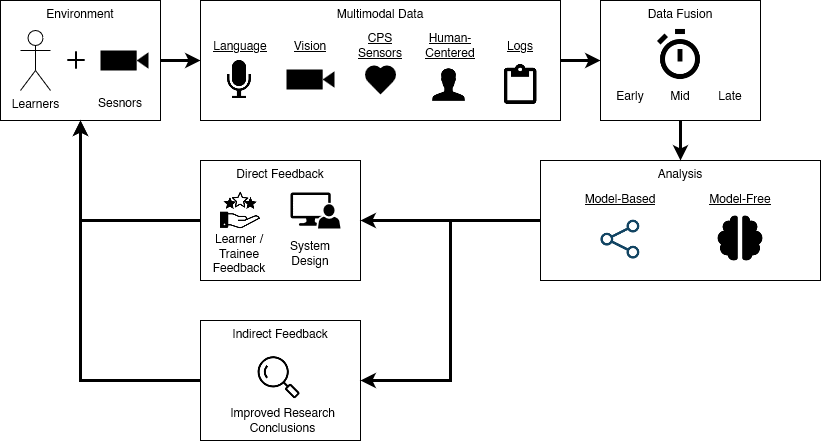
\includegraphics[width=0.9\textwidth]{img/MMLTE_Framework.png}
    \caption{MMLTE Survey Framework}
    \label{fig:framework}
\end{figure}

% Analysis RQs!

% Definitions:
%   Tables: feature name, description, mapped acronym
For the purposes of this paper, we define a \textit{modality} as a unique attribute defined by data from one of more datastreams, where each modality conveys different information, even if derived from the same data collection medium \cite{Ochoa?}. We define \textit{multimodal} as a combination of either multiple modalities or multiple datastreams (i.e., multiple data collection mediums). For instance, the same video datastream could be used for the affect and pose modalities (one-to-many), and the affect modality could be derived from separate audio and video datastreams (many-to-one). Both examples would be considered multimodal by our definition. Additionally, we use the terms ``papers" and ``works" interchangeably in this review, as we expand our definition of ``paper" to include other publications outside of conference and journal submissions (books, for example).
 
We define a \textit{learning environment} as any environment whose explicit purpose is to foster knowledge gain and retention. This can include school classrooms, tutoring centers, online learning environments like Khan Academy, etc. Learning environments are focused on helping users gain knowledge and retain information, and they are often (though not always) open-ended. We define a \textit{training environment} as any environment whose explicit purpose is to help users achieve an end goal, such as task-proficiency or a positive outcome other than learning. This is often done through practice and repetition, and can include military training, nursing training, physical training, workplace training, etc. Training environments are task-oriented and are often (though not always), constrained. 

Importantly, the question of what exactly constitutes ``multimodal" environments and analysis is debated. Some researchers argue that the term multimodal is defined by the uniqueness of a datastream (or sensor), meaning multiple modalities cannot be derived from the same datastream \cite{}. However, we consider multiple datastreams to be indicative of \textit{multimedia} and not multimodality \cite{}. Similar disagreements occur when defining what constitutes early versus late fusion and learning versus training environment. Additionally, not all multimodal learning and training environments are analyzed via multimodal methods. A \textit{multimodal composing} environment \cite{}, for example, may involve students creating works using multiple modalities (e.g., a comic book sketch with both text and images), but researchers may opt to only analyze students' discourse while in the environment (which would be unimodal analysis, and therefore outside the scope of this review). 

Consider a paper whose sole focus is multimodal composing environments that happens to perform multimodal analysis in passing. Should this paper be included in the search space, despite not having multimodal analysis as one of its foci? In this review, we argue yes, as we are interested in the different methods researchers are using to conduct multimodal analysis and are not limiting ourselves to only papers where multimodal analysis is a primary focus. Clearly, these distinctions are quite nuanced, which is why the definitions we use in this paper are not meant to be interpreted as ground truth. They were chosen, after much discussion, based on how we wanted to characterize the scope of our review.


\subsection{Environment Spectrum}\label{subsec:environmentSpectrum} % Physical <--- Mixed ----> Virtual

% Reminder that no AR/VR training environments that require learner to wear glasses in this study

One important aspect when considering the literature surrounding multimodal learning analytics (MMLA) is identifying the contexts in which these techniques are used, which mostly fall under the category continuum of learning and training (see Figure \ref{fig:ltcontinuum}). The main goals of learning environments are education and knowledge gain. These venues range from conventional classrooms to online courses and self-paced learning environments. When we categorize these environments on our continuum shown in Figure \ref{fig:ltcontinuum}, we add a second dimension, between fully physical and fully virtual, to represent this wide range of learning environments. MMLA methods applied in learning environments focus on extracting insights from various modalities such as text, audio, video, and interactions to assess students' comprehension, engagement, and progress. Educators may modify instructional tactics, spot problematic students, and improve learning materials by analyzing these multimodal signals since they provide significant insights into both individual and group learning patterns.

\begin{figure}
    \centering
    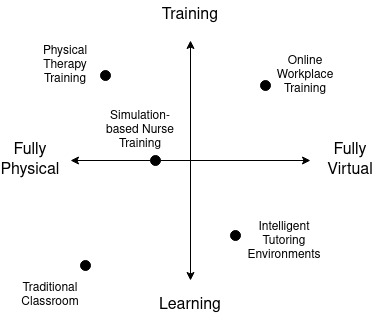
\includegraphics[width=0.5\textwidth]{img/LearningTrainingContinuum.jpg}
    \caption{Learning-Training Continuum}
    \label{fig:ltcontinuum}
\end{figure}

On the other hand, training environments are designed to improve performance and build skills. This category encompasses professional training programs, simulations, and vocational training platforms, across the same potential continuum of fully virtual to fully physical that we used to categorize learning environments. In training settings, MMLA approaches are used to evaluate data in order to track the mastery of new skills, the accomplishment of tasks, and overall performance. These insights help instructors and managers adjust training programs, spot competency gaps, and determine how prepared students are for issues in the real world. The objectives of MMLA differ in learning and training situations, calling for specific strategies that take into account the specifics of each situation, but in this paper we review literature across the spectrum of learning and training.

However, it is important to note that this division isn't always clear-cut. Some environments of study, like those populated by PhD students, blur the line between education and training. These students are learning new things in a vein similar to learning environments, but they are also increasing their research abilities and expertise, in a vein similar to a training program. Similarly, certain contexts, like game-playing platforms, defy easy classification into the learning or training categories. In these instances, MMLA methodologies must be flexibly applied, appreciating the multifaceted nature of the objectives at hand. In our categorization of all of the environments from our corpus of papers, we recognize this ambiguity in discrete categorization, but also recognize the utility of such a categorization when analyzing the research subcommunities that makeup the larger field of MMLA. As such, we perform a fuzzy qualitative discrete categorization based on discussions among the authors of where we believe each paper’s environment best fits on our continuum shown in Figure \ref{fig:ltcontinuum}.

\subsection{Data Collection Mediums} 
% Definitions reminders
% Researcher artifacts includes field notes and also labeling of the data (i.e., manual coding). 
% Participant artifacts includes pre/post tests and the like. To qualify, all artifacts must be collected and analyzed in the pipeline and cannot be collected post hoc afterward.
% Depth camera versus regular: discuss that both are video, but depth usually used for motion modality with skeletal features
% motion capture (posyx, accelerometer, gyroscope, magnetometer)
% Make point that things like learning gains and performance can fall into multiple categories depending on where derived from, e.g., logs, surveys, student artifacts (which can also be demo information)

% VID. Sequence of video frames from a camera source
% AUD. Audio signals captured and converted by a microphone
% SCREEN. Sequence of video frames of the contents displayed on a device screen
% EYE. Eye movement data and gaze points captured by a tracking devices with sensors and cameras 
% LOGS. Environment logs containing data on participants' activities and interactions within the system
% SENSOR. Specialized sensors used to gather participants' physiological data, such as photoplethysmography (PPG), electrodermal activity (EDA), and blood volume pulse (BVP)
% INTER. Structured or unstructured conversations between researchers and participants, i.e. interviews
% SURVEY. Standardized sets of questions administered to participants, such as surveys or questionnaires 
% PPA (Participant Produced Artifacts). Materials produced by research participants using different mediums, such as physical objects or pre/post test scores
% RPA (Researcher Produced Artifacts). Materials produced by the researchers which contribute to analysis and findings, such as field observation notes
% MOTION. Raw motion data collected by different devices/technologies, such as Inertial Measurement Units (IMU) or Ultra-Wideband (UWB) radio signals
% TEXT. Raw textual input


\subsection{Modalities} \label{sec:Modalities}
% Definitions

% AFFECT. The emotional state or affect exhibited by the participant
% POSE. The physical position or geolocation of the participant
% GEST. The gestures and body language displayed by the participant
% ACT. The observable actions or activities performed by the participant
% PROS. Prosodic speech information, including aspects like volume,  pauses, pitch, intonation.
% TRANS. Textual speech information obtained through speech transcription, i.e., speech-to-text
% QUAL. Qualitative researcher observations on the participant's behavior or environment
% LOGS. Data related to the research context and participant' activities, interactions, and performance within the system
% GAZE. Data on the direction and focus of the participant's eye gaze
% INTER. Notes from interviews between researcher and participant
% SURVEY. Responses to survey/questionnaire provided by the participant
% PULSE. The participant's pulse, indicating their heart rate
% EDA. Participant's electrodermal activity, measuring skin conductance as an indicator of arousal
% TEMP. Participant’s body temperature
% BP. Participant’s blood pressure 
% EEG. Participant's electroencephalography activity, recording brain electrical signals
% FATIG. The level of fatigue experienced by the participant during the activity
% EMG. Participant's electromyography activity, measuring muscle electrical signals
% PPA (Participant Artifacts). Artifacts produced by the participant
% RPA (Researcher Artifacts). Artifacts produced by the researcher
% SPECT (Audio Spectrogram). Visual representation of audio frequencies in the form of a spectrogram
% TEXT. Raw text data generated by the participant in the study environment
% PIXEL. Raw RGB pixel values representing visual information captured by cameras or sensors


\subsection{Analysis Methods}
% Definitions
% Pattern extraction analysis usually refers to identifying sequences, but can be other types of patterns (include examples, revisit later). Used as catch-all for when patterns are identified but do not fall under other subsets of pattern extraction like clustering. Sequwnce mining, some HMM applications, etc.
% Define classification for our purposes as using an algorithm to predict an output in a discrete space. Mention RL paper as using RL but falling into classification category by our definition. 
% Add caveat that analysis methods refers to analysis only of the data and not of the actual analysis, unless analysis of the analysis provides more information about the data (show examples)

% CLS (Classification)*.
% REG (Regression)*.
% CLUST (Clustering)*.
% QUAL (Qualitative)*.
% STATS (Statistical Methods). Statistical methods such as central tendency, ANOVA, correlation, etc. 
% NET (Network Analysis). Any analysis consisting of graph-based approaches, e.g. ENA.
% PATT (Pattern Extraction). Extracting patterns from data, such as sequence mining.


\subsection{Data Fusion}
% Graphic with different kinds of fusion
% Fusion definitions:
%   Early fusion. Raw, obserable data is fused directly from data collection medium and used for analysis. E.g. using raw audio signal and screen pixels, and fusing them for analysis.
%   Mid fusion. Observable features are unimodally extracted from raw data, and those extracted features are fused for analysis. E.g. extract affect from video and transcriptions from speech and fusing them for analysis. 
%   Add that we consider "cognitive load" an "observable" feature, as it comes out-of-the-box with some sensors' software (e.g. Kinect)
%   Late fusion. Unobservable features are extracted from the data, and then fused for analysis. E.g., fusing neural network output for analysis.
%   Explain: None or Other (OTH) fusion, hybrid fusion
%       cite Chango: A review on data fusion in multimodal learning analytics and educational data mining
%       "studies that do not fit into none of those three groups or in which the fusion point was not specified (Others category)"
%   Hybrid can either be separate pipelines (as traditionally defined) or multiple data types in the same pipeline

%   di mitri paper reference for observable/unobservable fusion definition: https://onlinelibrary.wiley.com/doi/full/10.1111/jcal.12288

In the realm of multimodal learning analytics (MMLA), data fusion plays a pivotal role in harnessing the power of multiple data sources to provide a more comprehensive and insightful understanding of the learning process. The process of data fusion involves combining information from various sources to create a unified dataset, thereby facilitating enhanced interpretation and analysis, when compared to analyzing only a single modality at a time. By combining data from multiple modalities, researchers and educators can uncover hidden insights into learners' cognitive states, emotions, and behaviors. This comprehensive understanding paves the way for personalized interventions and more effective pedagogical strategies. 

Within data fusion, the traditional method of categorization, as underscored by Chango et al.’s \cite{Chango2022} recent review of data fusion within MMLA, is based on three categories: early, late, and hybrid. The \textit{early fusion} approach involves combining raw data from multiple sources at the earliest stage of processing. This integration occurs before any individual modality-specific analysis, allowing for joint processing of data from different sources. By merging information early, the model can capture potential interactions and dependencies among modalities, but limited by cases where there are significant differences between data modalities and challenges surrounding the complexity and explainability of the joint modality models. The \textit{late fusion} approach involves performing separate analyses on individual modalities and then integrating their outcomes at a later stage. This method allows for specialized processing of each modality's characteristics, potentially leading to more accurate and contextually relevant insights, but limited in its ability to capture intermodal relationships that might exist. The \textit{hybrid fusion} approach aims to combine the strengths of both early and late fusion methods. In this approach, data from various sources are combined at multiple stages of processing. For instance, an initial early fusion step might be followed by separate analyses of each modality using a late fusion strategy. This allows for the exploitation of intermodal relationships while also accommodating the uniqueness of each modality's information. However, hybrid models increase the overall complexity of data analysis and require a priori decisions about which features should be combined at what points in the model pipeline. The choice of fusion method depends on several factors, including the specific problem domain, the characteristics of the available data, the desired level of interpretability, and the computational resources available.

However, we argue that this traditional three-state categorization is actually not informed enough to fully capture the complexity of multimodal analysis. After qualitative review of our paper corpus, we had significant difficulty categorizing analysis methods into just these three categories due to the ambiguity surrounding what constitutes \textit{raw features} compared to \textit{processed features}. For example, some researchers might classify the joint position data measured by a Microsoft Kinect camera as a raw feature, and thus permissible in early fusion, since it is available from the camera without any additional processing by the researchers. However, others might classify this as a processed feature, and thus a part of hybrid or late fusion, since the Kinect camera is actually computing this data from the raw depth data, regardless of whether this computation is obfuscated to the end user. Qualitatively, we noticed this pattern and disagreement among researchers with multiple modalities within our paper corpus. Motivated by this finding, we propose an additional category of data fusion, which we call \textit{mid fusion}. 

Mid-fusion represents a middle point between early fusion and late fusion, where data could be somewhat processed and transformed before being combined, but not transformed to the same extent as in late fusion. The difference here between mid and late fusion can be somewhat subtle depending on the modality, but is perhaps best explained using Di Mitri et al.’s \cite{DiMitri2018} conceptualization of the \textit{observability line}. In their work, modalities are categorized into \textit{input space}, which represents observable evidence and data that can be tracked with sensors, and \textit{hypothesis space}, which represents inferred learning labels. These two categories are separated by the \textit{observability line}, which they describe as "a line of separation between the observable evidence and all the possible interpretations" \cite{DiMitri2018}. In our new framework for categorizing data fusion, \textit{early fusion} represents combination without any initial processing, \textit{mid fusion} represents combination of features that have had prior processing that stays within the input space (i.e., still observable features), and \textit{late fusion} represents combination of features that have had prior processing that crosses the observability line into the hypothesis space (i.e., no longer directly observable).

For example, consider the same Kinect sensor discussed earlier. In this case, the raw pixel values from the camera image or the raw depth values from the depth sensor would be considered unprocessed observable features and candidates for early fusion. However, the joint position coordinates output by the camera SDK would be considered observable processed features, and thus candidates for mid fusion, since they are derived from other observable data, but still remain directly observable. Beyond this, if a researcher used the joint position data as input to another model which estimated a measure of motivation, for example, then this motivation construct would only be a candidate for late fusion, since we have now crossed the observability line. 

This classification is still somewhat qualitative and up to a researcher's interpretation. As described by Di Mitri et al., "The distinction between observable/unobservable is conceptual and can vary in practice." \cite{DiMitri2018}; however, we believe that this additional data fusion category helps to resolve some of the ambiguity related to the original categorization scheme and is useful for identifying the sub-communities of MMLA based on which methods researchers have applied. For a concrete definition of the modalities that we consider oberservable for the categorization in this paper, see section \ref{sec:Modalities}. In addition to the early, mid, late, and hybrid data fusion categories, in this paper, following the methodology of Chango et al. \cite{Chango2022}, we add an \textit{other} category to catch studies that do not fit into one of those four groups or in which the fusion point was not specified.

\subsection{Environment Setting}
% Confirm exact set from S18 corpus to be sure!
% Environment Setting. Physical, virtual, blended, unspecified.

\subsection{Environment Subject}
% Confirm exact set from S18 corpus to be sure!
% Environment Subject. STEM, humanities, psychomotor skills, other, unspecified

\subsection{Participant Structure}
% Confirm exact set from S18 corpus to be sure!
% Participant Structure. Individual, multi-person, unspecified


\subsection{Didactic Nature}
% Didactic Nature. Instructional, training, informal, specified 

\subsection{Level of Instruction or Training}
% Confirm exact set from S18 corpus to be sure!
% Level of Instruction or Training. K-12, university, professional development

\subsection{Analysis Approach}
% MB vs MF.

\section{Methods} \label{sec:methods} % How our literature view was done

% Overview of methods section to include lit search, study selection, feature extraction, and analysis methods

\subsection{Literature Search} \label{subsec:literature_search}

This literature review examines contemporary multimodal analytics methods applied to learning and training environments. Our aim is to collect all pertinent papers published between 1/1/2017 and 10/22/2022. The proceeding paragraphs detail the methods used to construct our literature corpus and the efforts taken to consider all relevant papers, which we then distill via both quantitative (network analysis) and qualitative (quality control) methods to a manageable amount of works we believe to be representative of the current state of the field. In doing so, we introduce a novel graph-based study selection approach that uses a directed citation graph to exclude irrelevant works based on a paper's incoming and outgoing citations. To the authors' knowledge, this approach has not been previously used for distilling a literature review corpus. Our procedure for performing the quality control portion of this literature review is adapted from Barbara Kitchenham's ``Procedures for Performing Systematic Reviews" \cite{kitchenham2004procedures}.

Our literature search consisted of 42 queries agreed upon and defined by the authors as being representative of the body of works this literature review would be conducted on. Instead of performing our queries manually, our approach leverages programmatic querying via API-based web scraping for Google Scholar. There are multiple tools for scraping Google Scholar information, such as \href{https://pypi.org/project/scholarly/}{scholarly} and \href{https://github.com/venthur/gscholar}{gscholar}. Ultimately, we employed \href{https://serpapi.com/google-scholar-api}{SerpAPI}, a proprietary third-party Google Scholar web scraping API, for its most essential feature: organic web results. Other API tools' results are not organic, i.e., a query made via the API and one manually queried in a browser-based environment will produce two different sets of results.

Queries were posed via API request to Google Scholar for papers published between 1/1/2017 and 10/22/2022 (the date of the literature search). 2017 was collectively agreed upon as being the best cutoff date for inclusion in our search due to the rapid technological advancements in the field over the past 5 years. Several papers prior to 2017 are discussed in Section \ref{sec:background}, as they are seminal works; however, they are not considered for inclusion in our corpus. 

For the literature search, this review's authors decided on 14 distinct search strings, and each string was searched 3 times with a different spelling of the word \textit{multimodal} --- multimodal, multi-modal, and multi modal --- prepended to it. The 14 search strings are enumerated in Table \ref{tab:search_terms}.\footnote{The term ``xai" was originally included in the search queries due to the authors' interest in exploring explainable AI methods applied to learning and training environments. Unfortunately, the field is still nascent, and no usable query results were returned given our search criteria.}

\begin{table}[htbp]
    \renewcommand{\arraystretch}{1.3}%
    \centering
    \caption{Search strings used for the literature search.}
    \begin{tabularx}{\linewidth}{l@{\hskip .25in} l@{\hskip .25in}}
    
        \midrule
        education technology & explainable artificial intelligence \\

        \midrule
        learning analytics & learning environments \\
        
        \midrule
        learning environments literature review & learning environments survey \\
    
        \midrule
        literature review & simulation environments \\
        
        \midrule
        survey & training environments \\
        
        \midrule
        training environments literature review & training environments survey \\
        
        \midrule
        tutoring systems & xai \\

        \bottomrule
    \end{tabularx}
    \label{tab:search_terms}
\end{table}

For each of the 42 queries, the top 5 pages (100 publications) deemed most relevant by Google Scholar were collected. The top-5 cutoff was financially imposed because of our subsequent citation graph construction (Section \ref{subsubsec:quantitative_pruning}). To build the citation graph, each individual paper's citation information is queried, but each query is capped at 20 citations per API call by SerpAPI. This means that a paper with 100 citations requires 5 additional API calls to gather all of its citation information. The number of API calls needed to construct the citation graph would be intractable (and unaffordable) if the initial search was left unbounded; therefore, the top-5 cutoff was put in place.

Our initial search yielded a total of 4,200 papers. The distillation procedure we used for corpus reduction is enumerated in Table \ref{tab:procedure} and discussed in the proceeding subsections. Throughout the section, each step of our corpus reduction procedure is identified via its Step ID in Table \ref{tab:procedure}.

\begin{table}[htbp]
    \renewcommand{\arraystretch}{1.3}%
    \centering
    \caption{Corpus reduction procedure. Step ID 0 is the literature search. Steps IDs 1-7 were performed quantitatively via pruning the initial search corpus's citation graph. Subsequent steps were performed qualitatively via our quality control procedures. At each step of the corpus reduction procedure, the number of papers pruned and number of papers remaining are listed.}
    \begin{tabularx}{\linewidth}{l@{\hskip .25in} l@{\hskip .25in} l@{\hskip .25in} l@{\hskip .25in}}
        Step ID & Procedure & Removed & Remaining \\
        \midrule
        
        0 & Literature search & 0 & 4200\\
        
        1 & Remove duplicates & 2079 & 2121\\

        2 & Remove non-English & 1 & 2120\\

        3 & Remove degree-0 nodes & 488 & 1632\\
        
        4 & Remove disconnected components & 101 & 1531\\
        
        5 & Iteratively remove degree-0 and degree-1 nodes & &\\

        \quad 5.1 & \quad Iteration 1 & 373 & 1158\\

        \quad 5.2 & \quad Iteration 2 & 74 & 1084\\
        
        \quad 5.3 & \quad Iteration 3 & 19 & 1065\\
        
        \quad 5.4 & \quad Iteration 4 & 2 & 1063\\

        6 & Remove titles with keywords & 204 & 859\\
        
        7 & Title reads & 471 & 388\\
    
        8 & Abstract reads & &\\
        \quad 8.1 & \quad Remove inaccessible abstracts & 10 & 378\\
        \quad 8.2 & \quad First abstract round & 211 & 167\\
        \quad 8.3 & \quad Second abstract round & 40 & 127\\

        9 & Full paper reads & & \\
        \quad 9.1 & \quad First full paper round & 52 & 75\\
        \quad 9.2 & \quad Feature discretization and extraction & 2 & 73\\
        \quad 9.3 & \quad Second full paper round & 0 & 73\\
        
        \bottomrule
    \end{tabularx}
    \label{tab:procedure}
\end{table}

Our initial corpus contained 2,079 duplicates, which were removed by hashing paper titles (Table \ref{tab:procedure}, Step ID 1). If a paper had multiple versions (or other duplicates), we used the official source (e.g., journal or conference) of publication. We removed 1 non-English paper (Table \ref{tab:procedure}, Step ID 2) due to pragmatism (English is the only language shared between all of the authors). Non-English papers were identified using \href{https://spacy.io/universe/project/spacy_fastlang}{spaCy FastLang}, where any paper whose title was identified as having less than a 100\% chance of being non-English was selected for manual review. In total, our initial search yielded 2,120 unique (English) papers published during or after 2017.

\subsection{Study Selection} \label{subsec:study_selection}
To reduce our corpus to a reviewable body of works, we employed both qualitative and quantitative methods. After the initial search, we distilled the corpus quantitatively via a citation graph, which is discussed in Section \ref{subsubsec:quantitative_pruning}. Subsequent distillation was performed via qualitative means and is discussed in Section \ref{subsubsec:quality_control} subsection. 

\subsubsection{Citation Graph (Quantitative Pruning).}\label{subsubsec:quantitative_pruning}

For visualization, analysis, and distillation purposes, we used \href{https://networkx.org/}{NetworkX} to create and display a citation graph of the initial 2,120 works considered for inclusion in this review. The graph is a directed acyclic graph (DAG), where each node is a paper uniquely identifiable by its UUID (universally unique identifier) on Google Scholar, and each directed edge from A to B indicates paper A cited paper B. For the purposes of this paper, we consider the degree of each node $n$ to be the sum of both incoming and outgoing edges, i.e. papers citing $n$ and papers cited by $n$, respectively. We again used SerpAPI for collecting the list of works that cited each paper. The citation search did not need to be conducted in both directions, as any paper citing another paper in our corpus would already have been identified by the ``cited by" list of the paper being cited. Citations by papers not included in our initial search (i.e., in the DAG) were ignored. Initially, our DAG contained a 3-node cycle. This was due to versioning and preprint overlap, as papers by the same author cited each other during preprint. Once the cycle was identified, its nodes' edges were updated, and the cycle was removed. No nodes were removed as a result of correcting the cycle.

Once the DAG was constructed, we removed all 0-degree nodes (Table \ref{tab:procedure}, Step ID 3) (i.e. nodes with no edges coming in or going out). We felt it reasonable that if a paper did not cite (or was not cited by) any other papers in the field as determined by our literature search, then the paper was either not relevant to the field or did not yield results or methods referenced by subsequent works. Importantly, this biases the corpus in favor of more recent works. Works from early 2017 may not have any outgoing edges simply due to being some of the earliest works in the corpus, which would have precluded these works from being able to cite any papers in the corpus because they had not yet been published. However, these same papers had a greater opportunity to be cited by subsequent papers, which is why we felt it important to consider both incoming and outgoing edges: we expect earlier papers to have more incoming edges and later papers to have more outgoing edges. Altogether, pruning 0-degree nodes from the DAG reduced our corpus by 488, dropping our count to 1,632 works.

After removing 0-degree nodes, we examined the DAG's connectivity (Table \ref{tab:procedure}, Step ID 4) to identify disconnected components not relevant to our literature search. This had to be done to account for overlapping terminology across domains. For example, a cursory look at our initial search results included several ``multimodal training" papers related to deep learning (DL), where artificial neural networks (ANNs) are trained using data across multiple modalities. Our expectation based on our search strings was the relevant works would comprise the largest component of the DAG, and other smaller, disconnected components could then be discarded as irrelevant because they lacked any edge to or from the DAG's primary component.

Evaluating the DAG's connectivity, we found one large component consisting of 1,531 nodes (papers) and 4 smaller, disconnected components of various sizes. The disconnected components totaled 101 papers. The node sizes of the disconnected components, their frequencies of occurrence in the DAG, and the total number of papers at each node size are listed in Table \ref{tab:disconnected}. 101 papers were removed by pruning disconnected components from the DAG, which left 1,531 papers represented by a single connected graph. 

\begin{table}[htbp]
    \renewcommand{\arraystretch}{1.3}%
    \centering
    \caption{Disconnected DAG components by number of nodes in the component (component size), frequency of occurrence, and total number of papers. For instance, the first row indicates that there were 35 disconnected components with 2 nodes in the graph, totaling to 70 papers.}
    \begin{tabularx}{0.5\linewidth}{l@{\hskip .25in} l@{\hskip .25in} l@{\hskip .25in}}
        Component Size & N Occurrences & Papers \\
        \midrule
        
        2    &  35 &  70\\
        \midrule
        
        3    &  6  &  18\\
        \midrule
        
        4    &  2  &  8\\
        \midrule
        
        5    &  1  &  5\\

        \bottomrule
    \end{tabularx}
    \label{tab:disconnected}
\end{table}

Once we had our connected graph, we removed 1-degree nodes to further prune it. This created new 0-degree nodes, which were also subsequently removed. This process of removing 1- and 0-degree nodes was repeated iteratively for a total of four iterations (Table \ref{tab:procedure}, Step ID 5) until the graph was stable (i.e., removing 1-degree nodes did not create any new 0-degree nodes). By iteratively removing 1- and 0-degree nodes, we felt we could effectively identify and remove works outside the scope of our literature review without losing works directly related to multimodal learning and training environments. This is because the field of multimodal learning and training environments spans several sub-fields across computer science, education, and cyberphysical systems, and the authors agreed it was unlikely papers with so few edges would be relevant to our review if they had not cited (or been cited by) more than a few other works in our corpus. We removed 373 nodes in the first iteration (Table \ref{tab:procedure}, Step ID 5.1), 74 nodes in the second iteration (Table \ref{tab:procedure}, Step ID 5.2), 19 nodes in the third iteration (Table \ref{tab:procedure}, Step ID 5.3), and 2 nodes in the fourth and final iteration (Table \ref{tab:procedure}, Step ID 5.4). Altogether, we removed 468 papers across four iterations, which reduced our corpus from 1,531 papers to 1,063. 

A cursory look at the remaining 1,063 titles informed us that a large part of our corpus was still outside the scope of our review. We first noticed many papers related to training multimodal neural networks, whereby neural networks are trained on multimodal datasets to perform multimodal tasks. An example of this is \textit{image captioning}, where a neural network is trained to write a caption for a given image \cite{yu2019multimodal}. This requires multimodal training, as the network must have knowledge of both vision and language. We also noticed many works applying multimodal methods to the medical field, usually in terms of imaging. Medical images take many forms, and multiple forms can be combined to train a deep learning model in a multimodal fashion. For example, Cheng at al. used both computed tomography (CT) and magnetic resonance (MR) images to train a neural network for deep similarity learning, where a binary classifier is trained to learn the correspondence between two image patches \cite{cheng2018deep}. To remove papers pertaining to multimodal neural network training and multimodal medical applications, we programmatically identified 217 titles via regex keyword search (Table \ref{tab:procedure}, Step ID 6) that contained at least one of six of the following words: neural, deep, machine, medical, medicine, and healthcare. We then evaluated the selected titles by hand. Of the 217, 13 were kept in the corpus due to their potential relevance to our review. Papers employing deep learning methods in multimodal learning analytics (MMLA) and applying multimodal methods to medical learning or training environments were within the scope of our review, for example. For reference, we removed one paper titled, ``deep learning for object detection and scene perception in self-driving cars: survey, challenges, and open issues" \cite{gupta2021deep}; and we kept one titled, ``supervised machine learning in multimodal learning analytics for estimating success in project‐based learning" \cite{spikol2018supervised}. The remaining 204 papers were removed from the corpus, reducing it to 859 potentially relevant works.

It was at this point we concluded our quantitative pruning procedures and began qualitatively reducing the corpus, which we discuss in the next subsection.

\subsubsection{Quality Control (Qualitative Pruning).} \label{subsubsec:quality_control}

After applying quantitative methods to prune the corpus via the citation graph, we employed qualitative methods to further reduce the dataset by hand. This involved selecting papers for exclusion based on consensus. Pursuant to Kitchenham \cite{kitchenham2004procedures}, we initially excluded works based on reading paper titles, then paper abstracts, and eventually full papers. The first five authors of the review acted as reviewers for the quality control procedure. 

For the title reads (Table \ref{tab:procedure}, Step ID 7), four of the reviewers read all 859 titles. For each title, each reviewer independently determined whether the title was likely to fall inside the scope of the review. The results were tallied, and papers were then selected for inclusion/exclusion based on majority voting, i.e., papers with at least three votes ``for" were automatically included, and papers with at least three votes ``against" were automatically excluded. For the papers with a 2-2 tie, a fifth reviewer was used as a tie breaker. The reviewers selected 347 papers for inclusion and 372 papers for exclusion. 140 papers were tied, and a fifth reviewer selected 41 of those for inclusion. In total, 388 papers were selected for inclusion after the title reads --- 347 by majority vote, and 41 by tie-breaker.

Before conducting the abstract reads (Table \ref{tab:procedure}, Step ID 8), several works were excluded due to their inaccessibility (Table \ref{tab:procedure}, Step ID 8.1). While gathering the abstracts, we noticed not all papers were publicly available. Several were defined by invalid URLs or behind paywalls. Whenever a paper's abstract (or introduction, in the case of a book) was unavailable via its SerpAPI URL, a Google search was conducted in order to obtain the abstract manually through websites such as ResearchGate\footnote{\href{https://www.researchgate.net/}{https://www.researchgate.net/}} and other academic repositories. When this failed, we relied on the Vanderbilt University Library's proxy to access papers behind paywalls. If we were unable to freely access a paper's abstract online through Google search or via Vanderbilt's proxy, the paper was excluded from the corpus. Altogether, 10 papers were removed due to inaccessibility, leaving 378 papers for the abstract reads.

The ``abstracts" quality control procedure consisted of two rounds. Similar to the  procedure for the title reads, each of the 378 abstracts from the remaining papers was first assigned to two reviewers, and a majority voting scheme was employed (Table \ref{tab:procedure}, Step ID 8.2). Papers were then selected for inclusion or exclusion based on a predefined set of exclusion criteria. The exclusion criteria for the abstracts is listed in Table \ref{tab:abstract_exclusion_criteria}. Exclusion criteria are cumulative, so each criterion applies to subsequent steps in our corpus reduction procedure. An exclusion criterion for the abstracts will similarly apply to full paper reads later on, for example.

\begin{table}[htbp]
    \renewcommand{\arraystretch}{1.3}%
    \centering
    \caption{Exclusion criteria for the abstract reads. Each of the 378 abstracts was assigned to two different reviewers. Each reviewer was instructed to exclude works based on this set of criteria.}
    \begin{tabularx}{\linewidth}{l@{\hskip .25in}}
        \midrule
        1. Paper does not deal with learning or training environments \\
        2. Paper's environment is VR-only \\
        3. Paper does not analyze multimodal data \\
        4. Paper does not apply multimodal analysis methods \\
        5. Paper is not original applied research\\
        \bottomrule
    \end{tabularx}
    \label{tab:abstract_exclusion_criteria}
\end{table}

Because this literature review focuses on multimodal methods applied to learning and training environments, any paper not dealing with a learning or training environment was not considered for this review. As mentioned in Section \ref{sec:intro}, VR environments were also not considered for inclusion in our corpus due to issues with scaling this technology in classroom settings and the lack of semantic meaning with respect to the environment for video analysis. If a paper does not analyze multimodal data, it is similarly out-of-scope for this review. In Section \ref{sec:intro}, we define multimodal analysis as analysis conducted on either multiple modalities or multiple datastreams. It is possible to have only one modality but be considered multimodal if that single modality is derived from multiple datastreams. To be included in our review, papers must also include systematic methods for analyzing the multimodal data, and those methods must be original, applied research. Papers that are literature reviews, pedagogical tools, theoretical foundations, doctoral consortiums, etc., may be used for reference in our Introduction and Background, but they are not considered for inclusion in the actual review corpus unless they additionally provide original, applied research via multimodal methods and analysis.

Of the 378 abstracts, reviewers agreed to keep 96 papers (i.e., both reviewers selected the work for inclusion) and discard 211 (i.e., both reviewers selected the work for exclusion). 71 were selected for further review (i.e., one reviewer selected the work for inclusion and one reviewer selected the work for exclusion). To address the 71 abstracts that did not receive unanimous agreement among reviewers, a second round of abstract reads was performed (Table \ref{tab:procedure}, Step ID 8.3) on the abstracts. This round consisted of each of the 71 abstracts without unanimous agreement receiving three additional reads: one read from each of the three reviewers who did not read the abstract in the initial abstract round. Each of the 71 papers was selected for inclusion based on a majority voting scheme (i.e., papers were kept if and only if at least two out of the three follow-up round reviewers elected to keep the abstract in the corpus). Of the 71 follow-up round papers, 31 were selected for inclusion, and 40 were removed from the corpus. With 96 papers selected for inclusion from the first round of abstract reads, and 31 papers selected from the second round, 127 papers in total were kept in the corpus for the next round of quality control: full paper reads.

Similar to the ``abstracts" quality control procedure, the ``full paper" quality control procedure also involved two rounds of review. To conduct full paper reads (Table \ref{tab:procedure}, Step ID 9), the 127 papers kept from the abstract round of quality control were split into 5 approximately equal partitions and randomly assigned to the 5 reviewers. Conducting full paper reads took several weeks, during which two additional exclusion criteria were defined. They are enumerated in Table \ref{tab:full_paper_exclusion_criteria}:

\begin{table}[htbp]
    \renewcommand{\arraystretch}{1.3}%
    \centering
    \caption{Exclusion criteria for the full paper reads. Each of the 127 papers was assigned to two different reviewers. Each reviewer was instructed to exclude works based on this set of criteria (in addition to the previously established exclusion criteria).}
    \begin{tabularx}{\linewidth}{l@{\hskip .25in}}
    
        \midrule
        
        1. Paper's results must be informative with respect to learning or training \\
        2. Paper's analysis methods must be able to be determined from the manuscript\\

        \bottomrule
    \end{tabularx}
    \label{tab:full_paper_exclusion_criteria}
\end{table}

Certain papers deal with learning or training environments but are outside the scope of this review because they are not informative with respect to learning or training. Consider a paper presenting a novel neural network architecture that uses a classroom dataset as a performance benchmark. While the classroom constitutes a learning environment, the paper itself is not conducting research to inform learning or training, but rather is using a dataset collected from a learning environment to inform its "core AI" research. We elected not to include these types of works in our review, as we aim to focus on multimodal methods that explicitly inform learning or training. Additionally, a few papers we encountered did not have analysis methods that were well-defined enough for feature extraction (i.e., we were unsure of their exact methods for analyzing the data). This often included short workshop papers whose method details were unable to be determined without referencing an external work\footnote{This does not include all workshop papers. Only those papers whose analysis methods could not be determined from the manuscript}. Because these types of papers would be very difficult to reproduce on their own, we elected to exclude them from our review.

During the first round of full paper reads (Table \ref{tab:procedure}, Step ID 9.1), all papers received one initial read. Reviewers marked each paper as ``immediate exclude," ''immediate accept," ``borderline exclude," or ``borderline accept." Papers marked as ``immediate exclude" were discussed by all 5 reviewers and excluded only if all agreed. These were papers with easily identifiable reasons for exclusion based on our criteria (for instance, a proposed theoretical framework with no analysis or a doctoral consortium presenting ideas for future research). No papers were ever excluded from our corpus during full paper reads without unanimous agreement from all five reviewers. Papers marked as ``immediate accept" were kept in the corpus for the second full paper read round. Papers marked as ``borderline exclude" or ``borderline accept" were assigned to a separate reader for further review and were subsequently discussed. Similar to papers marked for immediate exclusion, borderline papers were excluded prior to the second full paper read round only if all authors agreed. Altogether, 52 papers were excluded during the first round of full paper reads, which left 75 works remaining in the corpus. 

\subsection{Feature Extraction}

During the first full paper read round, several features were extracted from each paper (Table \ref{tab:procedure}, Step ID 9.2). Features included identifying information (e.g., title, first author, publication year), and information related to the paper's methods (e.g., data collection mediums, modalities, and analysis methods). The extracted features and their descriptions are found in Table \ref{tab:feature_extraction}.\footnote{For the ``Year" category, we used the date the manuscript was first publicly available (if listed, otherwise we used the publication date) in order to most accurately represent when the methods were performed. In some instances, the first date of online availability preceded the official publication date by over a year. Additionally, only data that was ultimately used in the paper's analysis was considered for the ``Data Collection Mediums" category (i.e., if it was collected but never analyzed, we did not include it).}

\begin{table}[htbp]
    \renewcommand{\arraystretch}{1.3}%
    \centering
    \caption{Features extracted from each paper.}
    \begin{tabular}{p{0.25\linewidth}@{\hskip .1in} | @{\hskip .1in}p{0.65\linewidth}@{\hskip .1in}}
        \toprule
        Feature & Description\\
        
        \toprule
        UUID & Universal unique identifier on Google Scholar.\\

        Title & Publication title. \\

        First Author & Publication's first author.\\

        Year & Year publication first publicly available.\\

        Environment Type & Type of environment analyzed in the publication.\\

        Data Collection Mediums & Devices and mediums used to collect and generate data from environment.\\

        Modalities & List of the different modalities used during analysis.\\

        Analysis Methods & List of the analysis methods used in the publication.\\

        Fusion Type & List of the types of data fusion used in the publication.\\

        Publication Source & Publication journal, conference, workshop, etc.\\
        
        \bottomrule
    \end{tabular}
    \label{tab:feature_extraction}
\end{table}

After the first read, the reviewers discussed their extracted features. To ensure alignment and understanding between all authors with respect to the features, feature categories were discretized via inductive coding \cite{}, where four of this paper's authors each extracted initial feature sets from 25\% of the corpus's papers. For example, the initially extracted data collection medium feature included instances of video camera, web camera, and Kinect camera, all of which were mapped to the ``VIDEO" data collection medium. Once the authors agreed on the discrete sets of features, papers were reread by their original reviewers, and their features were extracted into the discrete sets. The discrete feature-spaces are listed below in Table \ref{tab:circumscribing_features}. We call these features \textit{circumscribing features} to delineate them versus the identifying features (e.g., UUID, paper title, author, etc.) that were extracted for identification purposes but not used during analysis. 

\begin{table}[htbp]
    \renewcommand{\arraystretch}{1.3}%
    \centering
    \caption{Circumscribing features and their corresponding feature sets. For \textit{Environment Type}, items in the feature set are mutually exclusive (i.e., an environment can either be a learning \textit{or} training environment by our definition, but it cannot be both. All other circumscribing features can consist of multiple items in the feature set (e.g., each paper in our corpus will contain multiple mediums or modalities).}
    \begin{tabular}{p{0.22\linewidth}@{\hskip .1in} | @{\hskip .1in}p{0.45\linewidth}@{\hskip .1in}}
        \toprule
        Circumscribing Feature & Feature Set\\
        
        \toprule
        Environment Type & learning, training\\
        Data Collection Mediums & video, audio, screen recording, eye tracking, logs, physiological sensor, interview, survey, participant produced artifacts, researcher produced artifacts, text\\
        Modalities & affect, pose, gesture, activity, prosodic speech, transcribed speech, qualitative observation, logs, gaze, interview notes, survey, pulse, EDA, body temp, blood pressure, EEG, fatigue, EMG, participant artifacts, researcher artifacts, audio spectrogram, text, pixel value\\
        Analysis Methods & Classification, regression, clustering, qualitative, statistical methods, network analysis, pattern extraction \\
        Fusion Type & Early, mid, late, hybrid, none or other\\

        \bottomrule
    \end{tabular}
    \label{tab:circumscribing_features}
\end{table}

% Needs to be filled in with tables.
Each item in each of the circumscribing feature sets is described in Tables \ref{} (Environment Type), \ref{} (Data Collection Mediums), \ref{} (Modalities), \ref{} (Analysis Methods), \ref{} (Fusion Type), \ref{} (Environment Setting), \ref{} (Environment Subject), \ref{} (Environment Features), \ref{} (Analysis Goal), and \ref{} (Analysis Results).

During discretized feature extraction, additional papers were newly identified for possible exclusion pursuant to our aforementioned criteria. After discussing each paper selected for possible exclusion, 2 papers were removed from the corpus due to all five reviewers agreeing that each paper violated at least one exclusion criterion. After the two removals, 73 papers remained in the corpus, all of whose features were extracted into discrete sets pursuant to Table \ref{tab:feature_extraction} by the first full paper read round reviewer. At this point, a second and final quality control round was performed for full paper reads (Table \ref{tab:procedure}, Step ID 9.3), where each of the 73 papers remaining in the corpus was assigned to a reviewer who had not yet read that particular paper. For this round, reviewers were instructed to perform two tasks: identify any papers remaining in the corpus that violated any of the exclusion criteria (to discuss later for possible exclusion), and perform a round of feature extraction (to determine inter-rater reliability (IRR) with respect to the initial feature extraction via Cohen's $k$ \cite{cohen1960coefficient}). For this round, no additional papers were identified for exclusion, resulting in a final corpus of 73 works. Each paper's discrete feature sets were ultimately determined via consensus coding \cite{} by the two reviewers who read that particular paper (i.e., both reviewers needed to agree on the presence or absence of each feature in each paper). For reference, Cohen's $k$ before consensus was $k=0.873$.  

Once our corpus was finalized, we performed one additional round of feature extraction to extract additional circumscribing features to be used in our analysis. These features are: Environment Setting, Environment Subject, Participant Structure, Didactic Nature, Level of Instruction, Analysis Approach, and Analysis Results. All of these features are explained in Table \ref{} alongside their discrete values. The one exception is Analysis Results, which was not discretized due to the wide degree of variability across each paper's findings. Instead, we noted each paper's findings, and used them in our qualitative analysis via a thematic analysis \cite{}. The additional features were selected for extraction to allow for greater insight into the corpus via a more in depth analysis.

Similar to our initial round of feature extraction, we began with inductive coding, where four of this paper's authors first extracted the new circumscribing features for the same papers he or she performed inductive coding on during the previous round of feature extraction. We then discussed each paper's extracted features and formulated discrete sets for the new circumscribing features (with the exception of Analysis Results). During the first round of IRR, reviewers revisited the same papers they read during inductive coding and extracted the new circumscribing features pursuant to the agreed-upon feature sets devised during inductive coding. During the second round of IRR, reviewers reread (and extracted the additional features from) the same set of papers they were the 2$^{nd}$ reviewer for during the initial round of feature extraction. At this point, for each paper, the two reviewers who extracted that paper's additional features performed consensus coding to define that paper's final set of features. For reference, Cohen's $k=0.71$ for the additional round of feature extraction.

\subsection{Analysis Procedure}
% Explain analysis procedure pursuant to framework


\section{Findings}


\subsection{Environments}


\subsubsection{Setting}
% SOTA
% Challenges
% Research gaps

% Descriptive statistics for:
%   Environment type
%   Environment setting


\subsubsection{Learners}
% SOTA
% Challenges
% Research gaps

% Descriptive statistics for:
%   Participant structure
%   Level of instruction
%   Environment subject
%   Didactic Nature

\subsubsection{Data}
% SOTA
% Challenges
% Research gaps

% Descriptive statistics for:
%   Data Collection Mediums

\subsection{Multimodal Data}
% Descriptive statistics for:
%   Modalities

% One modality paper with 2 data collection mediums, vid and aud: 
\cite{3809293172}

% Thematic analysis cite: https://psycnet.apa.org/record/2011-23864-004

\begin{figure}
        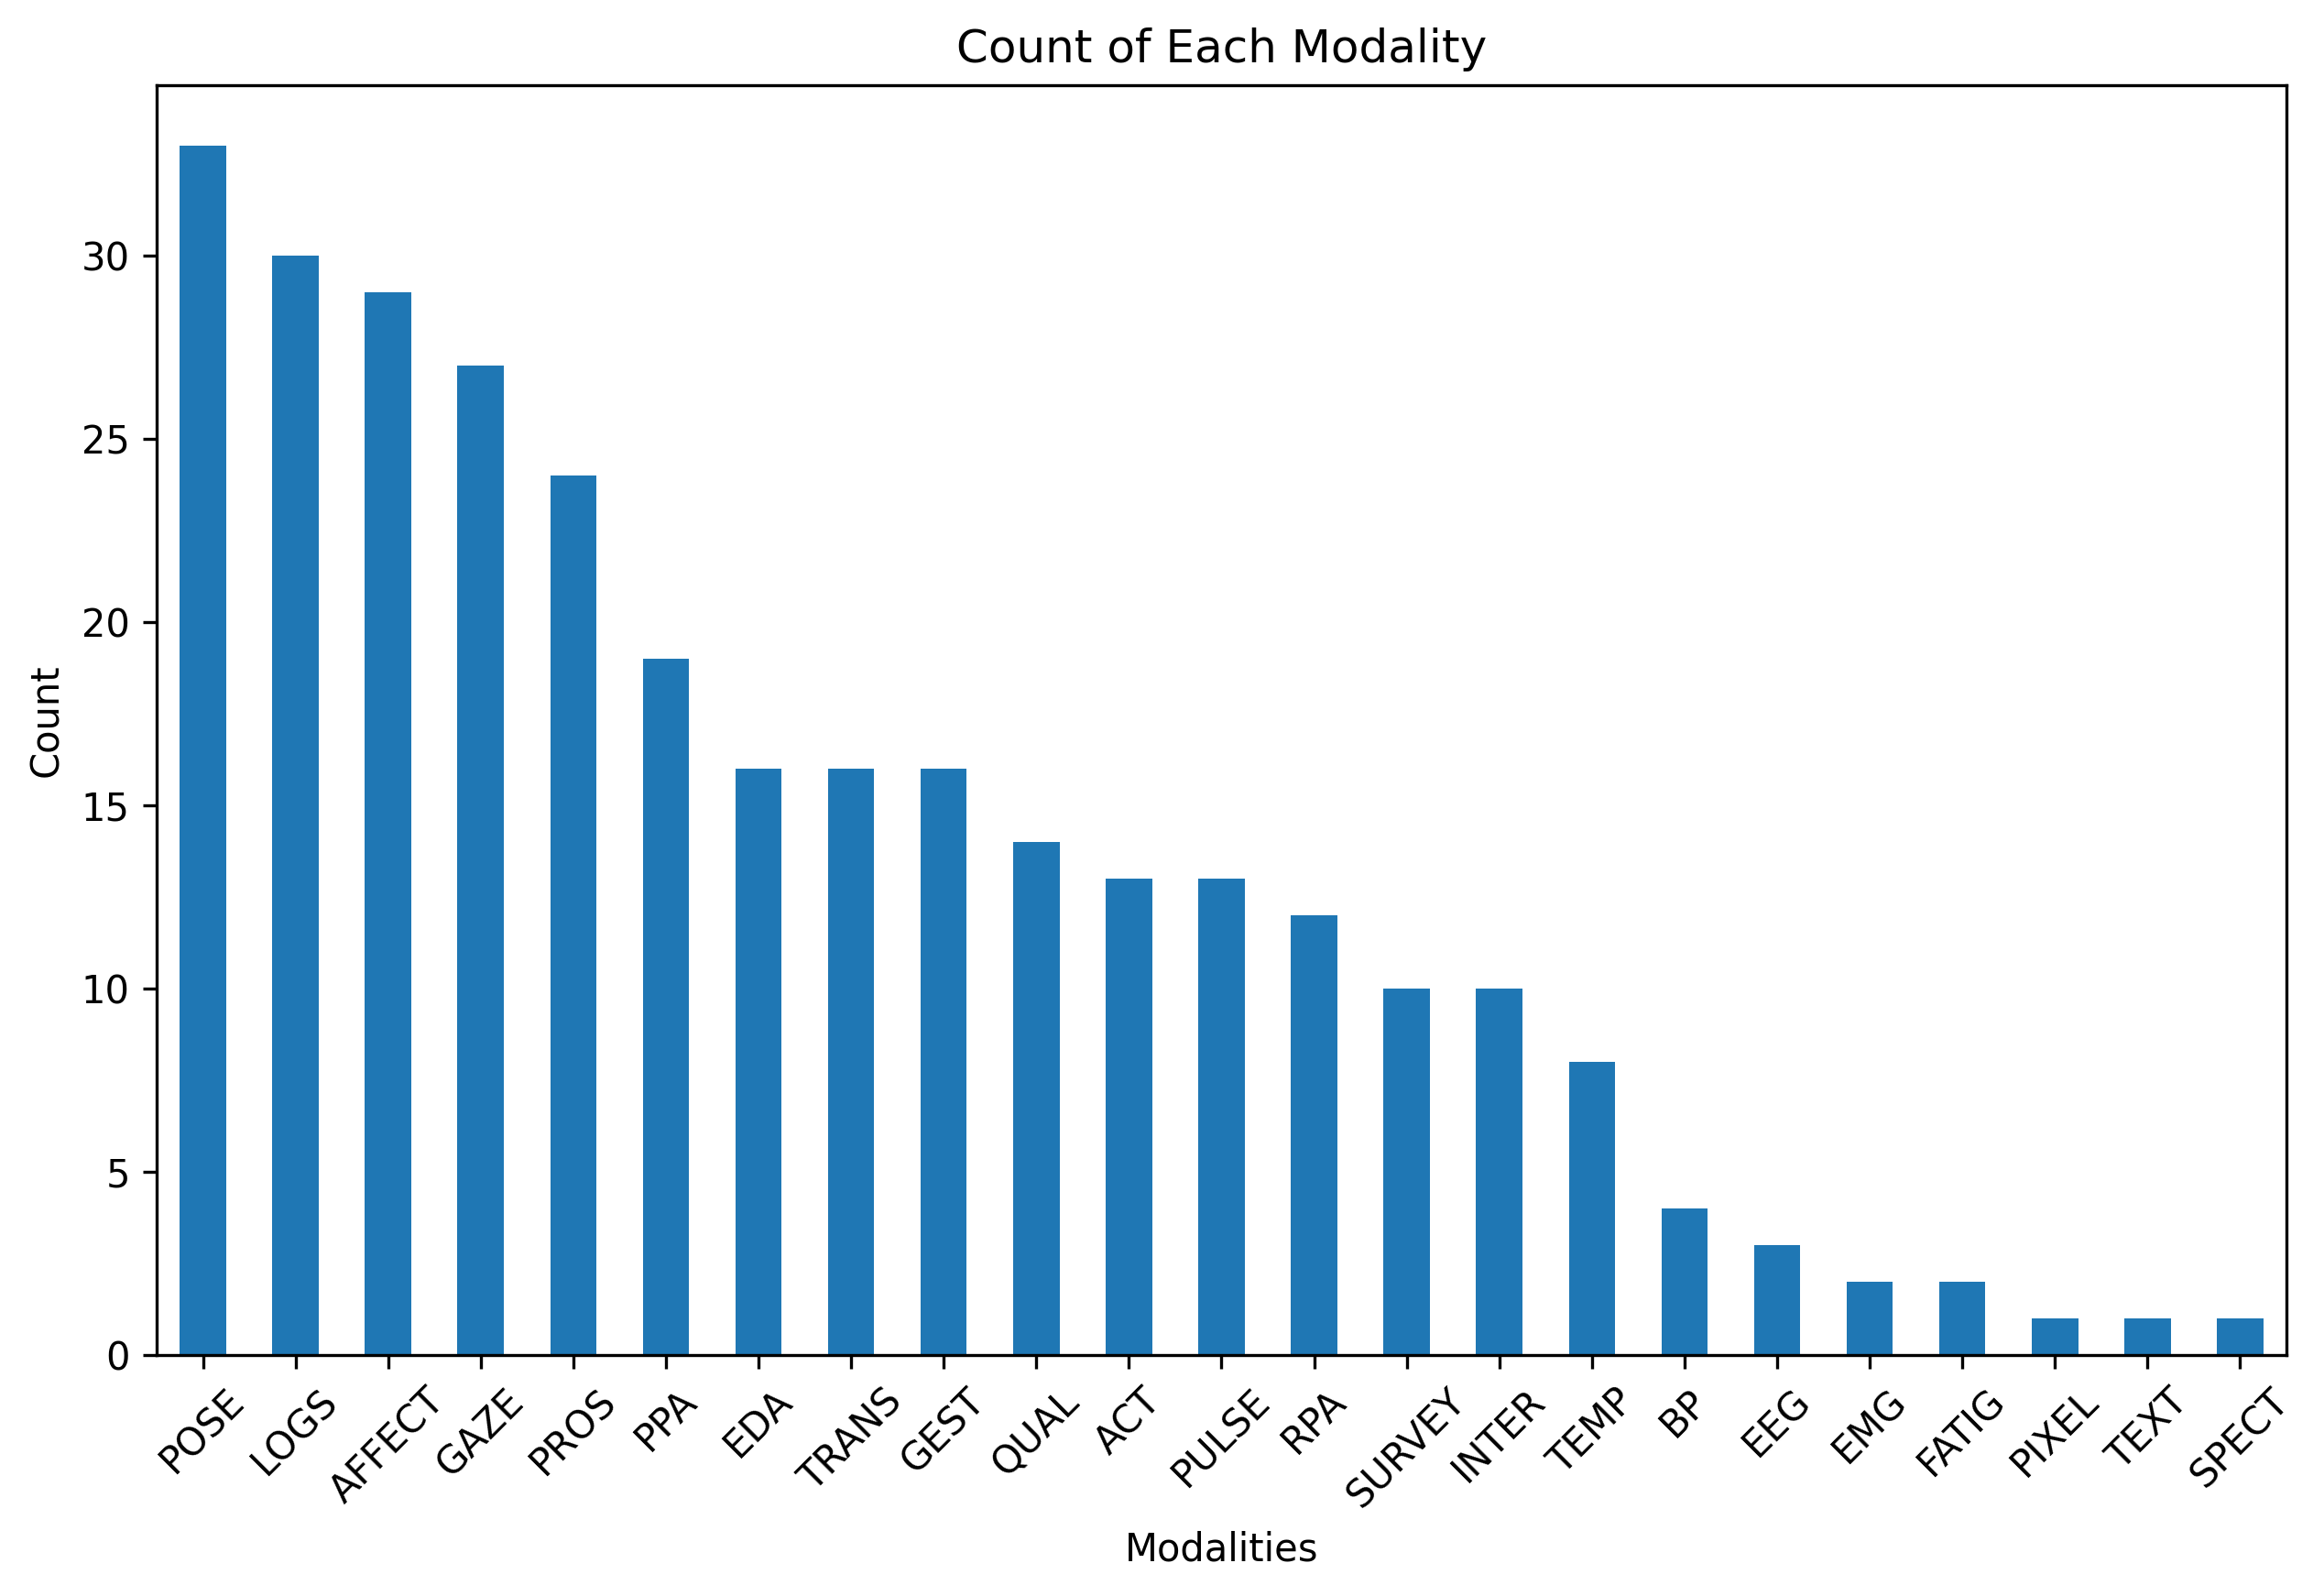
\includegraphics[width=\textwidth]{img/statistical_imgs/modalities.png}
        \caption{Modalities}
        \label{fig:modalities}
\end{figure}

\begin{figure}
        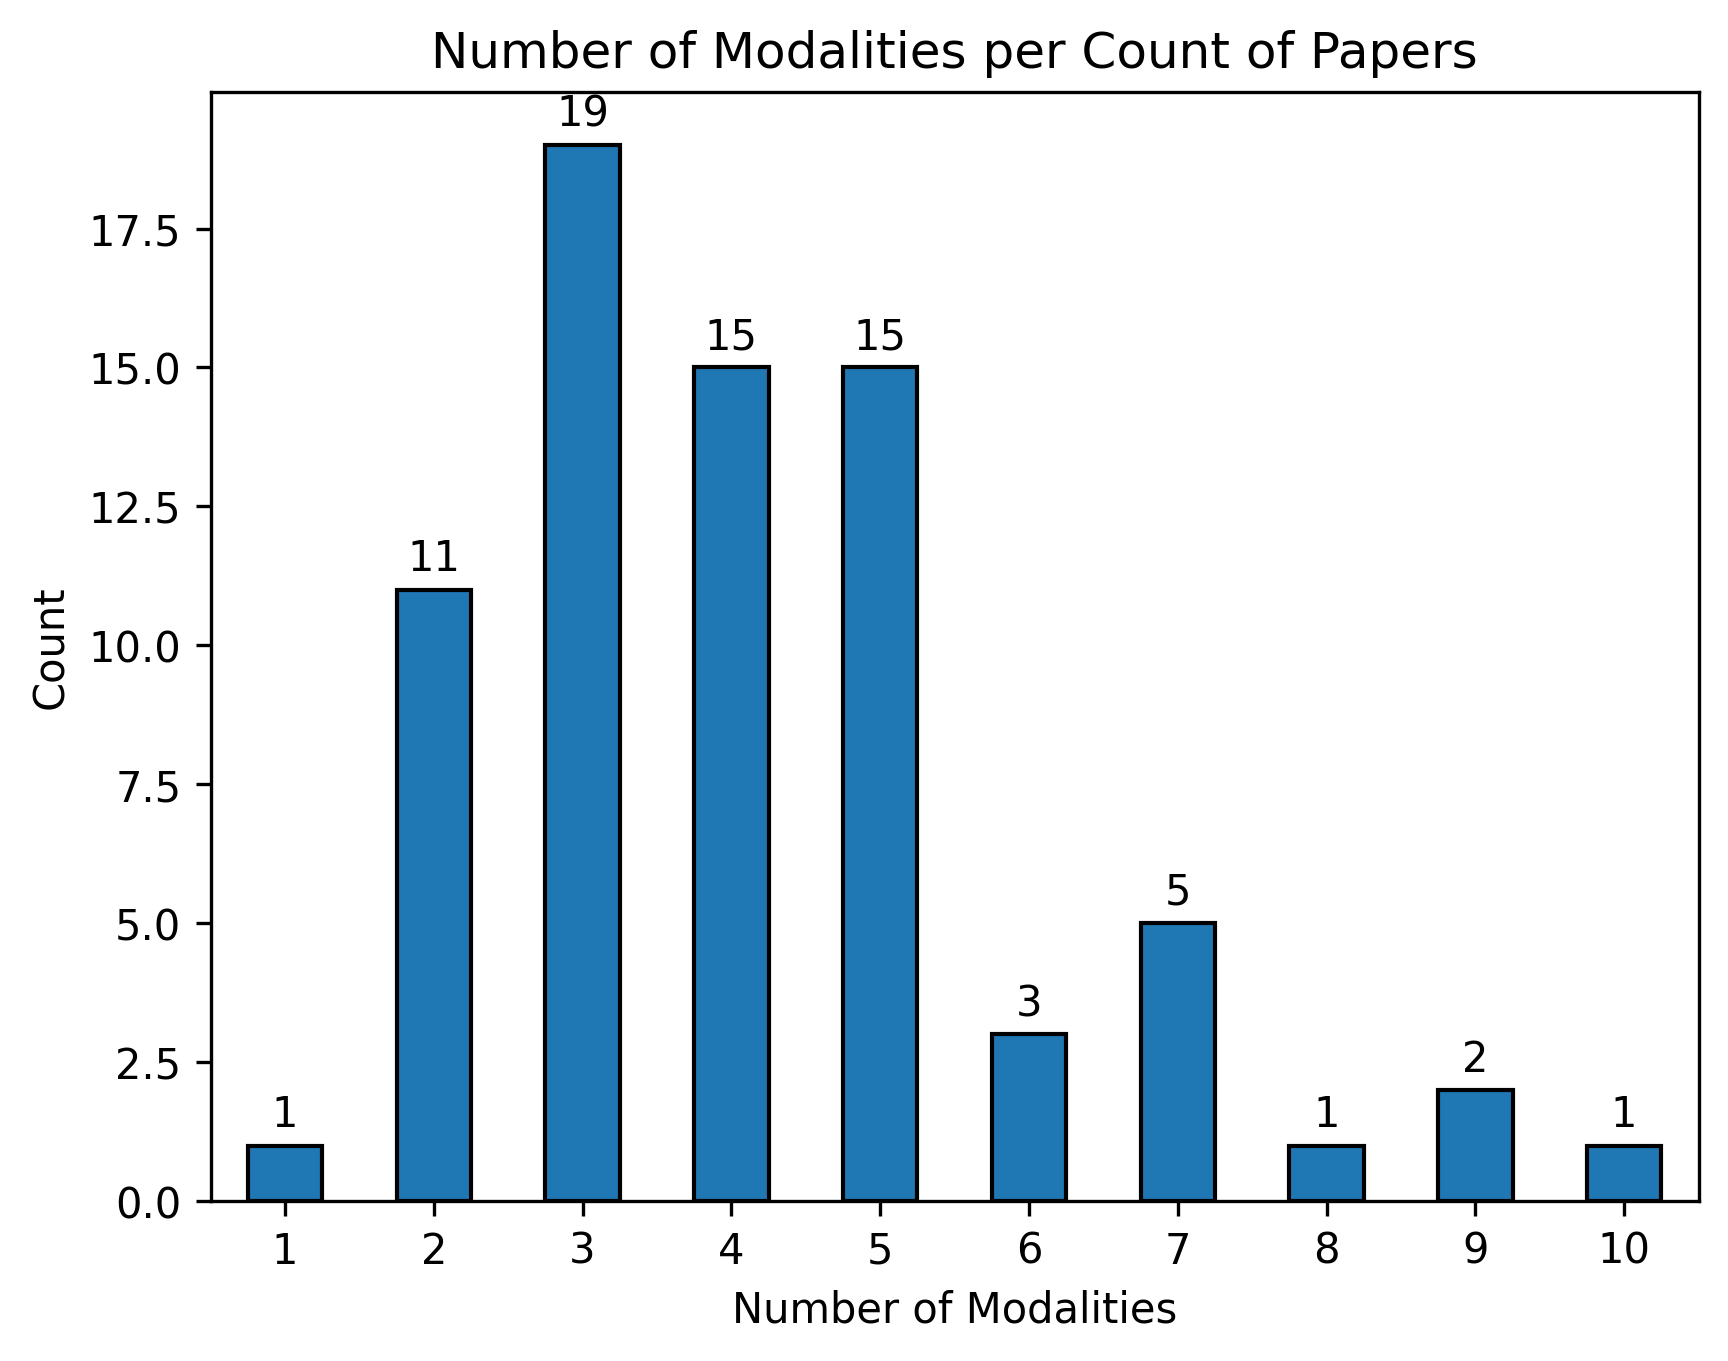
\includegraphics[width=\textwidth]{img/statistical_imgs/number of modalities per count of papers.png}
        
        % Add footnote about the 1 paper with only 1 modality having multiple data collection mediums, so we consider it multimodal by our definition.
        
        \caption{Modalities quantities}
        \label{fig:modalities_nums}
\end{figure}

% Introduce subdomains

\subsubsection{Natural Language}
% List # of papers falling into this subdomain
-35 papers use some form of natural language\\

% List Modalities
% PROS, TRANS, TEXT, SPECT, AFFECT
-PROS: 24\\
-TRANS: 16\\
-TEXT: 1\\
-SPECT: 1\\
-AFFECT: 2

Vast majority used prosodic audio and transcribed speech. Only 1 for raw text and 1 for audio spectogram.

Only 8 papers combine PROS and TRANS, and 24 use only one or the other. 

Most analysis is done via qualitative analysis and statistical methods. Some is done via classification, but not much with reg/patt/net. Contrast to full corpus, where classification was the most prevalent.
%NLP: {'REG': 6, 'CLS': 14, 'STATS': 21, 'CLUST': 3, 'QUAL': 19, 'PATT': 4, 'NET': 4}

% ALL: {'CLUST': 9,'QUAL': 29,'CLS': 39,'REG': 12,'STATS': 34,'PATT': 9,'NET': 4}

Only 9 papers in the entire corpus \textit{only} perform qualitative analysis. 7 of those papers use natural language in some form.
% Qual only: 
% NLP: 7/35
% ALL: 9/73

Fusion defined in 21/35 papers (60\%) with MID being the favorite. This is less prevalent than the fusion breakdown in the corpus, where ~75\% of papers define fusion (54/73). 
% NLP: {'MID': 12, 'EARLY': 1, 'OTH': 15, 'HYBRID': 5, 'LATE': 3}
% OTH fusion only fusion type in 14/35 papers

% ALL: {'HYBRID': 19, 'LATE': 8, 'MID': 27, 'EARLY': 3, 'OTH': 20}
% Full corpus OTH fusion only fusion type in 19/73 papers

No trend among environment settings really except virtual environments less frequent than blended/physical relative to full corpus. Suggests focus on collab in at least some physical space and not 1-on-1 agent interaction, for exanple.
% NLP: {'PHYS': 13, 'VIRT': 13, 'BLND': 8, 'UNSP': 1}
% ALL: {'BLND': 20, 'PHYS': 21, 'VIRT': 31, 'UNSP': 2}

Even with 4:3 ratio of ind to multi in corpus overall, ratio of ind to multi drops to 3:5 with NLP only due to focus on multiperson environments, including conversation. Not surprising given discourse component, but would also be interested in agent-based conversations (which were lacking). 
% NLP: {'MULTI': 23, 'IND': 14}
% ALL: {'IND': 45, 'MULTI': 31}

No trend among didactic nature. relative to overall corpus.
% NLP: {'INSTR': 21, 'TRAIN': 8, 'INF': 6}
% ALL: {'INSTR': 45, 'INF': 12, 'UNSP': 1, 'TRAIN': 15}

Both university and K12, although slight edge to K12 relative to corpus as a whole.
% NLP: {'UNI': 14, 'K12': 17, 'PROF': 3, 'UNSP': 4}
% ALL: {'K12': 30, 'UNI': 36, 'UNSP': 7, 'PROF': 5}

NLP has higher level of model free relative to corpus (17/41, 41\% relative to 27/57, 32\%)
% NLP: {'MB': 24, 'MF': 17}
% ALL: {'MB': 57, 'MF': 27}

% Results achieved
    -key feature ID relative to outcome (i.e., learning/training gains, skills, confidence, behaviors, strategies, collaboration quality, etc.) (e.g., pauses, n-grams, volume, pitch variation, etc.)
    -multimodal > unimodal

% SOTA 

-Data visualization (cite ChimeraPy IEE Big Data) 

-ML models are the most common quantitative approach: SVM, RF, Logistic regression, linear regression, NB, etc.
    -Usually used to regress/classify outcome (i.e., performance gains for learning/training)
    -Other methods used, but sparingly: clustering, behavior patterns, social network analysis, markov chains, etc.
    -AI methods lacking. DNN methods such as, RNN, LSTM, BERT...but rarer
    -Traditional NLP methods TF-IDF/Word2Vec used as baselines but not as part of the actual method

-Qualitative mostly involved descriptive statistics, case studies/individual observations, thematic analysis/constant comparative method of field notes/surveys, qualitative coding

-Stats: mostly correlation between features and specific features/feature combinations to outcome, and significance testing

-Lots of collaboration work, evaluating it both on its own and relative to outcome

% Challenges
-Hardware/software/multimodal and NLP method limitations for complex tasks (such as characterizing persuasive speech and understanding natural, oral arguments in debate)
    -Noisy, chaotic environments
    -ASR mentioned several times
        -Esp. with adolescents and in noisy environments (cite LID, LAK)
        -English only
        -"state-of-the-art diarization system does not perform well on real child-speech interactions"
    -Speaker diarization
-Data
    -Small datasets 
    -Jargon with domains/children (cite thesis)
-Complexity
    -Feature space: "From the audio data, 6405 features were extracted"
-Opaqueness
-Time   
    -Extensive preprocessing and feature engineering required
    -"a researcher may need to watch screen video data, listen to the audio dialogue several times, and enter behavioural codes into a separate document. Having to do this for every problem and concept students experience over the course of even one class period of learning technology use would be vastly taxing on human time and effort."
    -"we decided to split the audio manually, which was time consuming and, therefore, led to a lower number of students considered in the applied example."
-Temporality
    -Difficult to inform as it unfolds over time
    -segmentation
        -"difficulties segmenting the audio files in order to obtain the students-only utterances"
        
% Research gaps
-Lack of textual input. Discuss
-Only 8 papers use both transcribed audio and prosodic information, which means there is a lack of combining the two
    -Textless NLP lack with combined audio semantics/prosodic audio
-Focus on statistical analysis, qualitative, older ML, but lacking in SOTA AI (esp. RL, Transformers, although BERT/Audeering mentioned)
-Lack of conversational agent-based work. The stuff that's in there doesn't deal with actual conversations between students and agents, as the agent often acts as an evaluator and provides performance metrics or canned responses (i.e., 1-way recommendations) that are not robust to fluid environments  --- and does not act as a mentor, peer, or collaborator.

\subsubsection{Vision}
% List # of papers falling into this 
- 59 papers use some form of vision (Camera or Eye Tracking data collection medium with a mapped modalitiy in [POSE, AFFECT, GEST, ACT, FATIG, PIXEL, GAZE])

% List Modalities
% POSE, AFFECT, GEST, ACT, FATIG, PIXEL, GAZE
- 'GAZE': 27,
- 'FATIG': 2,
- 'ACT': 11,
- 'AFFECT': 25,
- 'POSE': 33,
- 'GEST': 16,
- 'PIXEL': 1

Vast majority of papers use some combination of GAZE, AFFECT, and POSE when analyzing video. A few use GEST and ACT. Only 2 and 1 papers use FATIG and PIXEL respectively. Lack of papers using PIXEL directly indicates 2 things: (1) Need for mid-fusion, as most people are not looking at raw image features; (2) Lack of alignment between core-vision SOTA and MMLA SOTA

Methods dist: \{'PATT': 8, 'NET': 2, 'QUAL': 24, 'CLUST': 7, 'CLS': 33, 'REG': 8, 'STATS': 26\}

No significant differences in the distributions of analysis methods between the complete dataset and the vision subset.

Approximately 10 papers did only QUAL or QUAL+STATS --- suggests that vision MMLA research is very computationally focused rather than only Qual focused. Further re-inforces by slightly higher percentage of model-based methods in vision compared to the overall dataset ($69.5\% vs 63.0$)

Vast majority of the total papers that apply QUAL methods (29) apply it using vision (24). Not surpising given the importance of analyzing video in qualitative research.

Almost no papers do early fusion using video data --- further support for the need of MID fusion

% SOTA
% Challenges & Research Gaps
Almost no papers are doing EARLY fusion using vision data -- suggests that everyone is relying on pre-trained unimodal vision models to perform multimodal inference. This is sensible, since training vision models is difficult and requires a lot of data, but also means there is potential performance improvements in these models by exploring fusing data early. Some examples of this are starting to come out in the CoreML field (e.g., CLIP variants), so it is a promising direction to explore.

Only 14 out of the 59 papers using Vision did a significant combination of qualitative and quantitative analysis --- most commonly a combination of classification and qualitative analysis of those classes. Suggests that much of the vision work is method papers, rather than aimed at understanding students more holistically. More researchers should explore mixed-methods approaches. 

% Results achieved
    % Advantages of multi-modal over uni-modal
\subsubsection{Sensors}
% List # of papers falling into this subdomain
% List Modalities
% AFFECT, POSE, EDA, PULSE, ACT, BP, TEMP, EEG, EMG, FATIG, GAZE
\textbf{Utilization of Wearable Sensory Data in the Matched Studies}

1. Monitoring Emotional and Physiological States: Many studies use wearable sensors to track physiological responses (heart rate variability, skin temperature, EDA) and correlate them with emotional states (e.g., stress, arousal) during learning activities like coding workshops and classroom environments.

2. Behavior and Performance Prediction: Wearable sensors, in combination with other modalities like eye-tracking and Kinect cameras, are used to predict behaviors like effort in assessments, performance in CPR training, and engagement in game-based learning.

3. Real-time Feedback and Adaptation: In studies like CPR training, wearable data is used to provide real-time feedback. Also, in classroom environments, data from wearables is used to adaptively recommend learning activities.

4. Multimodal Data Integration: Several studies integrate data from wearables with other sources, like Kinect-based posture data and facial cameras, for a comprehensive analysis of the learning process.

\textbf{Challenges Identified in These Studies}

1. Data Integration and Interpretation: Combining and interpreting data from various sensors and modalities to provide meaningful insights is a recurring challenge.

2. Balancing Accuracy and Practicality: Ensuring that the data collected is both accurate and practically useful for real-time applications, such as in CPR training feedback.

3. Contextual Relevance: Ensuring that the sensor data is relevant and accurately reflects the learning context, especially in dynamic and interactive environments like game-based learning or collaborative tasks.

4. Technical Limitations and Complexity: Dealing with the technical complexities of processing and analyzing multimodal data streams, especially when employing advanced machine learning techniques.

\textbf{State-of-the-Art Techniques in These Studies}

1. Advanced Predictive Modeling: Using machine learning and AI techniques, like support vector machines, deep neural networks, and reinforcement learning for predictive analysis.

2. Real-Time Feedback Systems: Developing systems that can process sensor data in real-time to provide immediate feedback, as seen in CPR training.

3. Effective Multimodal Data Fusion: Employing sophisticated data fusion techniques, such as feature-level concatenation, for enhanced predictive accuracy.

\textbf{Potential Gaps and Future Directions}

1. Long-Term Impact Analysis: Most studies focus on immediate or short-term effects; long-term studies to assess the sustained impact of these technologies are needed.

2. Broader Demographic and Contextual Application: Expanding research to include diverse learning contexts and demographic groups to understand the broader applicability of these technologies.

3. Scalability and Generalizability: Research often happens in controlled environments; scaling these technologies for widespread use and ensuring their generalizability remains a challenge.

4. User Experience and Acceptance: More research is needed on how learners perceive and interact with these technologies, especially in terms of comfort, usability, and perceived effectiveness.
Notes: \textbf{Storytelling With Learner Data: Guiding Student Reflection on Multimodal Team Data: To me this is the most interesting one, because of its realistic application in real world; the data seems limited and does not have IMU data and the data was logged by observer can be treated as ground truth. A more sophisticated model should be implemented.}

\textbf{More in-depth:}

\textbf{Missing Data-Driven Methods to Utilize Wearable Sensory Data}

\begin{enumerate}
    \item \textbf{Granular Data Analysis}: There's a need for more sophisticated data-driven methods that can delve into the finer details of wearable sensor data, such as identifying subtle patterns or correlations that might not be apparent with traditional analysis techniques.
    \item \textbf{Contextual and Behavioral Analytics}: Advanced analytics that can contextualize sensor data in real-time learning scenarios, linking physiological responses to specific learning activities or cognitive processes.
\end{enumerate}
\textbf{Lack of Visualization of Sensory Data}

\begin{enumerate}
    \item \textbf{Interactive Data Visualization}: Current studies often lack robust visual representations of the data collected from wearables. Interactive and intuitive visualizations can aid in understanding complex datasets, revealing patterns and trends in physiological responses and their triggers.
    \item \textbf{Visual Correlation with Learning Events}: Visualizing how sensor data aligns with specific learning events or actions can provide deeper insights into the learning process, such as identifying triggers for stress, engagement, or confusion.
\end{enumerate}
\textbf{Lack of Usage in Explainable AI (XAI) Methods}

\begin{enumerate}
    \item \textbf{Attribution-Based Methods}: The application of XAI, particularly attribution-based methods, is not extensively explored in these studies. Such methods could offer clarity on how different input features (sensor data) contribute to the model's predictions, enhancing the interpretability of AI-driven analyses in educational research.
    \item \textbf{Transparency in AI Models}: Incorporating XAI could also help in demystifying the decision-making process of AI models, especially when these models are used for predictive analytics or adaptive learning systems.
\end{enumerate}

% SOTA
% Challenges
% Research gaps

% Results achieved
    % Advantages of multi-modal over uni-modal
\subsubsection{Human-Centered}
% List # of papers falling into this subdomain

-TOTAL PAPERS\textbf{ 45} of 73 (QUAL or INTER or SURVEY or RPA or PPA)

% List Modalities
% QUAL 14, INTER 10, SURVEY 10, RPA 12, PPA 19

- QUAL 14, INTER 10, SURVEY 10, RPA 12, \textbf{PPA 19}

-Out of 45 papers, \textbf{0 have all 5} modalities, \textbf{1 has 4} modalities, \textbf{3 have 3} modalities, \textbf{11 have 2} modalities, \textbf{30 have 1} modality of the 5 (QUAL 6, INTER 3, SURVEY 6, RPA 6, PPA 9)

-Modalities that appear more frequently together: QUAL + PPA paired in 4 papers, PPA + RPA paired in 4 papers, INTER + QUAL paired in 4 papers

-Only 1 of 45 papers doesn't have other non-human-centered modalities (it is a paper that does clustering and regression using only RPA)

- Looking at analysis methods for the 45 papers: \textbf{STATS 22}, CLS 8, \textbf{QUAL 14}, CLUST 5, PATT 7, REG 5, NET 2: using human-centered data for statistical and qualitative analysis predominantly

\noindent\rule{2cm}{0.4pt}

Out of the 73 papers in your corpus, 45 (approximately 61.6\%) incorporate at least one of the human-centered modalities (QUAL, INTER, SURVEY, RPA, or PPA). This indicates a significant proportion of papers in your corpus that involve human-centered data collection methods. This concentration implies a strong interest in capturing and analyzing data that directly involves human experiences, perspectives, and artifacts, from the perspective of the human who produces the data based on its own interpretations of the tasks taking place during the activity.

Among the human-centered modalities, Participant Artifacts (PPA) has the highest representation with 19 papers, followed by Qualitative Researcher Observations (QUAL) with 14 papers and Researcher Artifacts (RPA) with 12. Interview Notes (INTER) and Survey responses (SURVEY) both have similar representation with 10 papers. 

The prevalence of Participant Artifacts (PPA) suggests a notable emphasis on utilizing materials produced directly by the study participants. This includes a diverse range of materials, depending on the nature of the study. The high count of Qualitative Researcher Observations (QUAL) indicates a focus on qualitative insights drawn directly from the researcher's observations of participant behavior and the environment.


% SOTA
-SOTA:

% Challenges
- Challenges: While a human-centered approach in multimodal learning analytics brings valuable insights, it also poses several challenges related to subjectivity, scalability, resource intensiveness, and potential limitations in generalizability. Due to the inherent subjectivity of human-centered modalities, the analysis of this data may be susceptible to the influence of the researcher's perspective, possibly introducing bias into the interpretation. Furthermore, these approaches often are resource-intensive, requiring trained researchers for data collection and analysis. Manual collection and human analysis can be time-consuming and may not scale well, especially in large-scale educational settings. Nevertheless, human-centered approaches may offer more transparent and interpretable insights than automated methods.

% Research gaps
-Research gaps:

% Results achieved
    % Advantages of multi-modal over uni-modal
- Advantages of multi-modal: By integrating multiple modalities, researchers can gain a more comprehensive understanding of the learning environment. This human-centered approach offers insights into the participants' experiences, perceptions, and behaviors, often pinpointing subtle nuances that might be missed in a unimodal analysis. QUAL provides rich contextual observations, PPA and RPA offer tangible artifacts, INTER captures in-depth discussions, and SURVEY provides multiple participant perspectives, collectively enriching the analysis. The use of multiple modalities allows for triangulation and cross-verification, where findings from different sources are compared to enhance the validity of the results.
    
\subsubsection{Logs}
% List # of papers falling into this subdomain
30 papers that use LOGS for their modalities analysis (40\% of the entire corpus). Log modality/medium stem from traditional LA and its role in contextualizing complementary data, along with video and audio.

% List Modalities
Since LOGS is its own modality and medium, I list below the counts of complimentary modalities:
-GAZE: 30 (13\%)\\
-AFFECT: 15 (12\%)\\
-POSE: 14 (11.4\%)
-EDA: 8 (7.3\%)
-PPA: 8 (7.3\%)
-RPA: 7 (6.5\%)
-ACT: 6 (4.8\%)
-PULSE: 5 (4\%)
-TEMP 5 (4\%)
-TRANS: 5 (4\%)
-QUAL: 5 (4\%)
-SURVEY: 4 (3.2\%)
-INTER: 4 (3.2\%)
-GEST: 4 (3.2\%)
-BP: 3 (2.4\%)
-EEG: 2 (1.6\%)
-FATIG: 2 (1.6\%)
-TEXT: 1 (0.8\%)
The distribution of complementary modalities matches that of the entire corpus.

% Analysis: QUAL vs QUANT
Logs are slightly used more in quantitative and mixed methods, yet relatively close to the corpus as a whole.
% {'QUANT': 12, 'MM': 11, 'QUAL': 7}
% {'QUANT': 40.0, 'MM': 36.67, 'QUAL': 23.33}
% {'MM': -5.80, 'QUANT': 3.01, 'QUAL': 2.78}

% Fusion
No early, largely because AI methods aren't trained to raw logs.
% {'mid': 11, 'hybrid': 10, 'oth': 7, 'late': 4}
% {'mid': 34.38, 'hybrid': 31.25, 'oth': 21.88, 'late': 12.5}
% {'mid': -0.70, 'oth': -4.09, 'hybrid': 6.57, 'late': 2.11, 'early': -3.9}

% Environment Setting
Except for 1 physical study, most of the log corpus generates their logs from computer-based systems where the end-user has a direct interface. 
% {'virtual': 16, 'blended': 12, 'physical': 1, 'unspecified': 1}
% {'virtual': 53.33, 'blended': 40.0, 'physical': 3.33, 'unspecified': 3.33}
% {'virtual': 11.44, 'physical': -25.05, 'blended': 12.97, 'unspecified': 0.63}

% Participant Structure
Within log-generating learning systems, individual activities compose 70\% of the corpus, compared to multi-person activities. Digital collaborative environments impose higher engineering and development costs; thereby, computer-based and blended studies heavily focus on individual students' trace logs.
% {'individual': 21, 'multi-person': 9}
% {'individual': 70.0, 'multi-person': 30.0}
% {'individual': 10.79, 'multi-person': -10.79}

% Didactic Nature
No trends in didactic nature related to the general corpus.
% {'instructional': 18, 'informal': 7, 'training': 5}
% {'instructional': 60.0, 'informal': 23.33, 'training': 16.67}
% {'instructional': -1.64, 'training': -3.88, 'informal': 6.89, 'unspecified': -1.37}

% Level of Instruction or Training
Logs are heavily used in undergrad population, with similar trends across different instruction levels.
% {'undergraduate': 17, 'k-12': 9, 'graduate': 4, 'k12': 3, 'unspecified': 1}
% {'undergraduate': 50.0, 'k-12': 26.47, 'graduate': 11.76, 'k12': 8.82, 'unspecified': 2.94}
% {'undergraduate': 10.47, 'k-12': -0.27, 'graduate': 0.13, 'k12': 0.68, 'unspecified': -5.20, 'professional development': -5.81}

% MB vs MF
More model-based methods compared to model-free with respect to the general corpus.
% {'model-based': 23, 'model-free': 9}
% {'model-based': 71.88, 'model-free': 28.12}
% {'model-based': 4.019999999999996, 'model-free': -4.02}

% SOTA (TODO)
- Learning outcomes:
    - Predicting learning variables (ML)
    - Student subtyping
- Cognitive and Metacognitive Analysis:
    - Sequence analysis (Markov)

% Challenges
- Time alignment (less combined with other hard-to-align modalities like physiological signals)
- Learning environment-dependent analysis
- Generalizability constraints
- High barrier entry to computer-based collaborative environments

% Research gaps
- Log standards exist to improve generalizability but are not referenced/used. [CITATION NEEDED]
- Results reproduction, transferring methods across different learning environments and contexts.
- Visualizations of logs data to important end-users (teachers)
- Low integration with EdTech (LTI, LMS, LXP)

% Results achieved
    % Advantages of multi-modal over uni-modal
\subsection{Data Fusion}


\subsubsection{Early Fusion}
% SOTA
% Challenges
% Research gaps

\subsubsection{Mid Fusion}
% SOTA
% Challenges
% Research gaps
    % Discuss the need for mid-fusion relative to early fusion

% Descriptive statistics for:
%   Fusion Types

\subsubsection{Late Fusion}
% SOTA
% Research gaps


\subsection{Analysis}
% SOTA
% Challenges
% Research gaps

% Descriptive statistics for:
%   Analysis Methods
%   Analysis Approaches (MB v. MF)
% Add plots here


\subsubsection{Model-Based}
% Obtain profiles for MB and MF corpus

\subsubsection{Model-Free}
% Obtain profiles for MB and MF corpus


\subsection{Feedback}

\subsubsection{Direct Feedback}
% SOTA
% Challenges
% Research gaps

% Learner/trainee feedback
% Online versus offline

\subsubsection{Indirect Feedback}
% SOTA
% Challenges
% Research gaps

% System design
% Improved research conclusions
% Online versus offline

\begin{figure}[h!]
    \centering

    % Commented out because no longer using
    
    % \begin{subfigure}[b]{0.45\textwidth}
    %     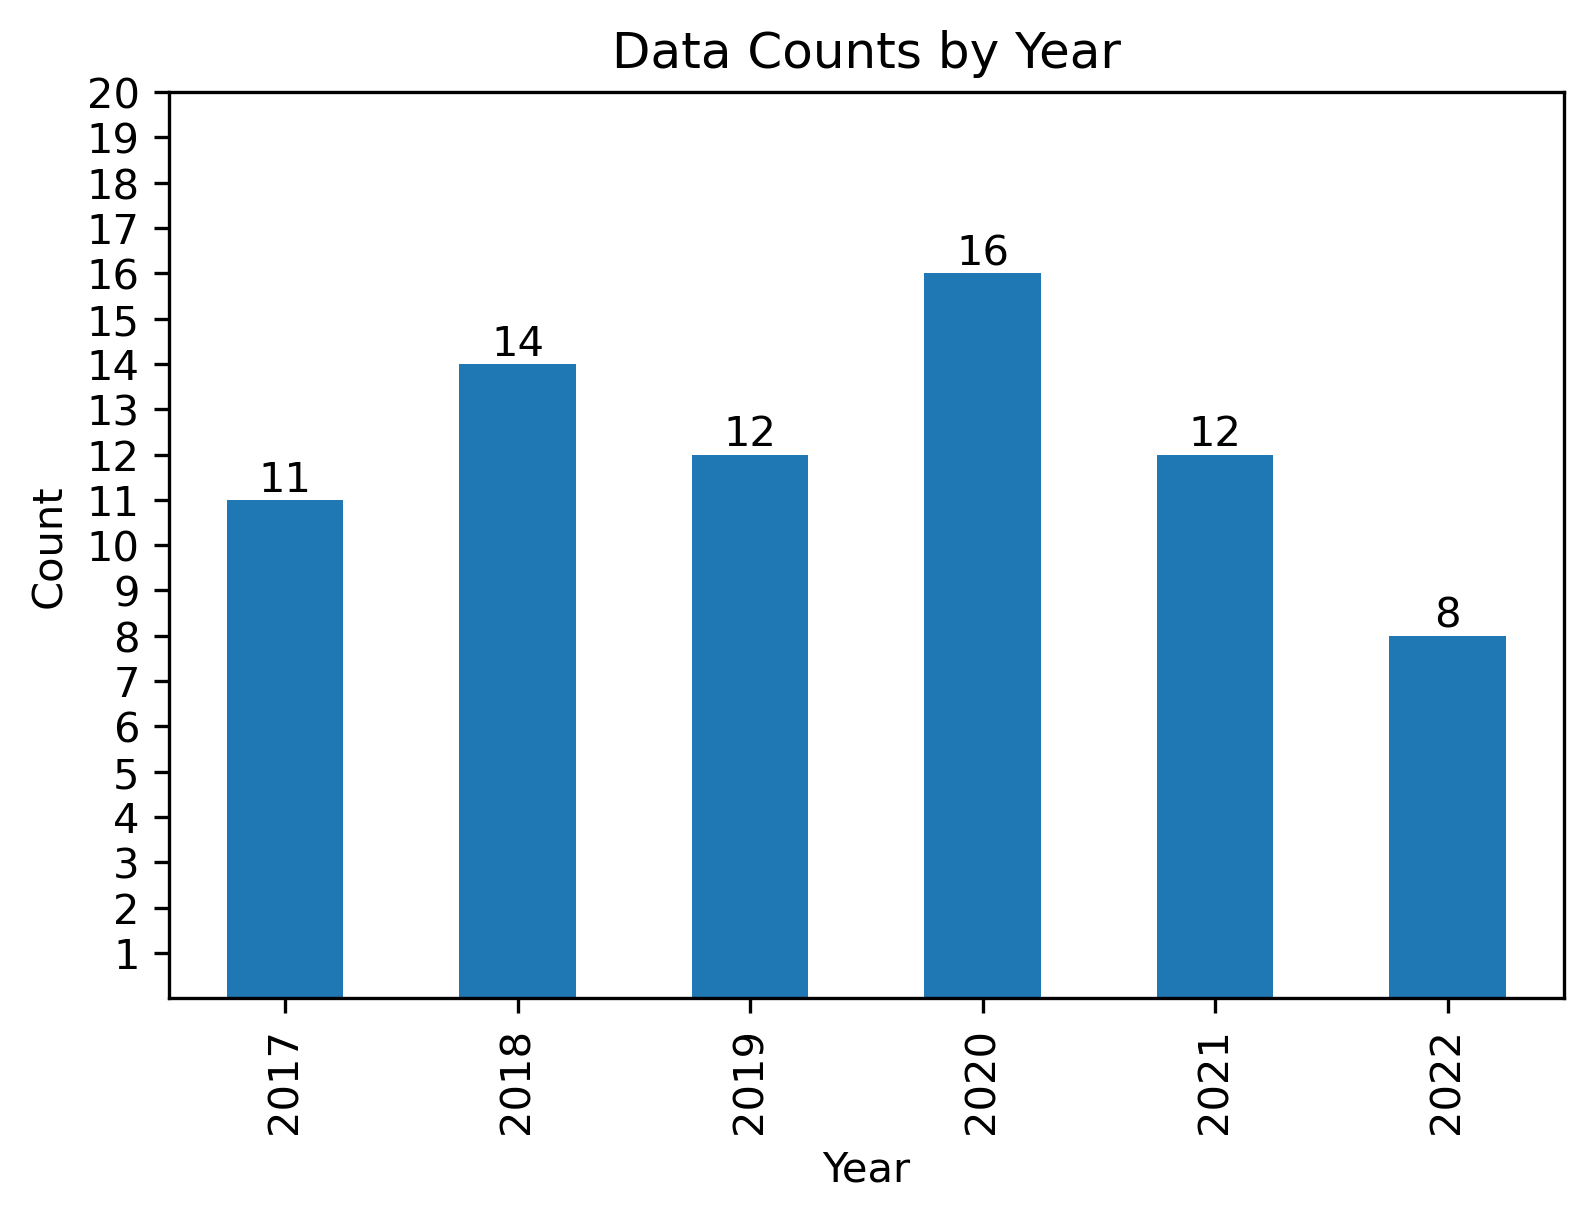
\includegraphics[width=\textwidth]{img/statistical_imgs/year.png}
    %     \caption{Image 1}
    % \end{subfigure}
    % \hfill
    
    \begin{subfigure}[b]{0.45\textwidth}
        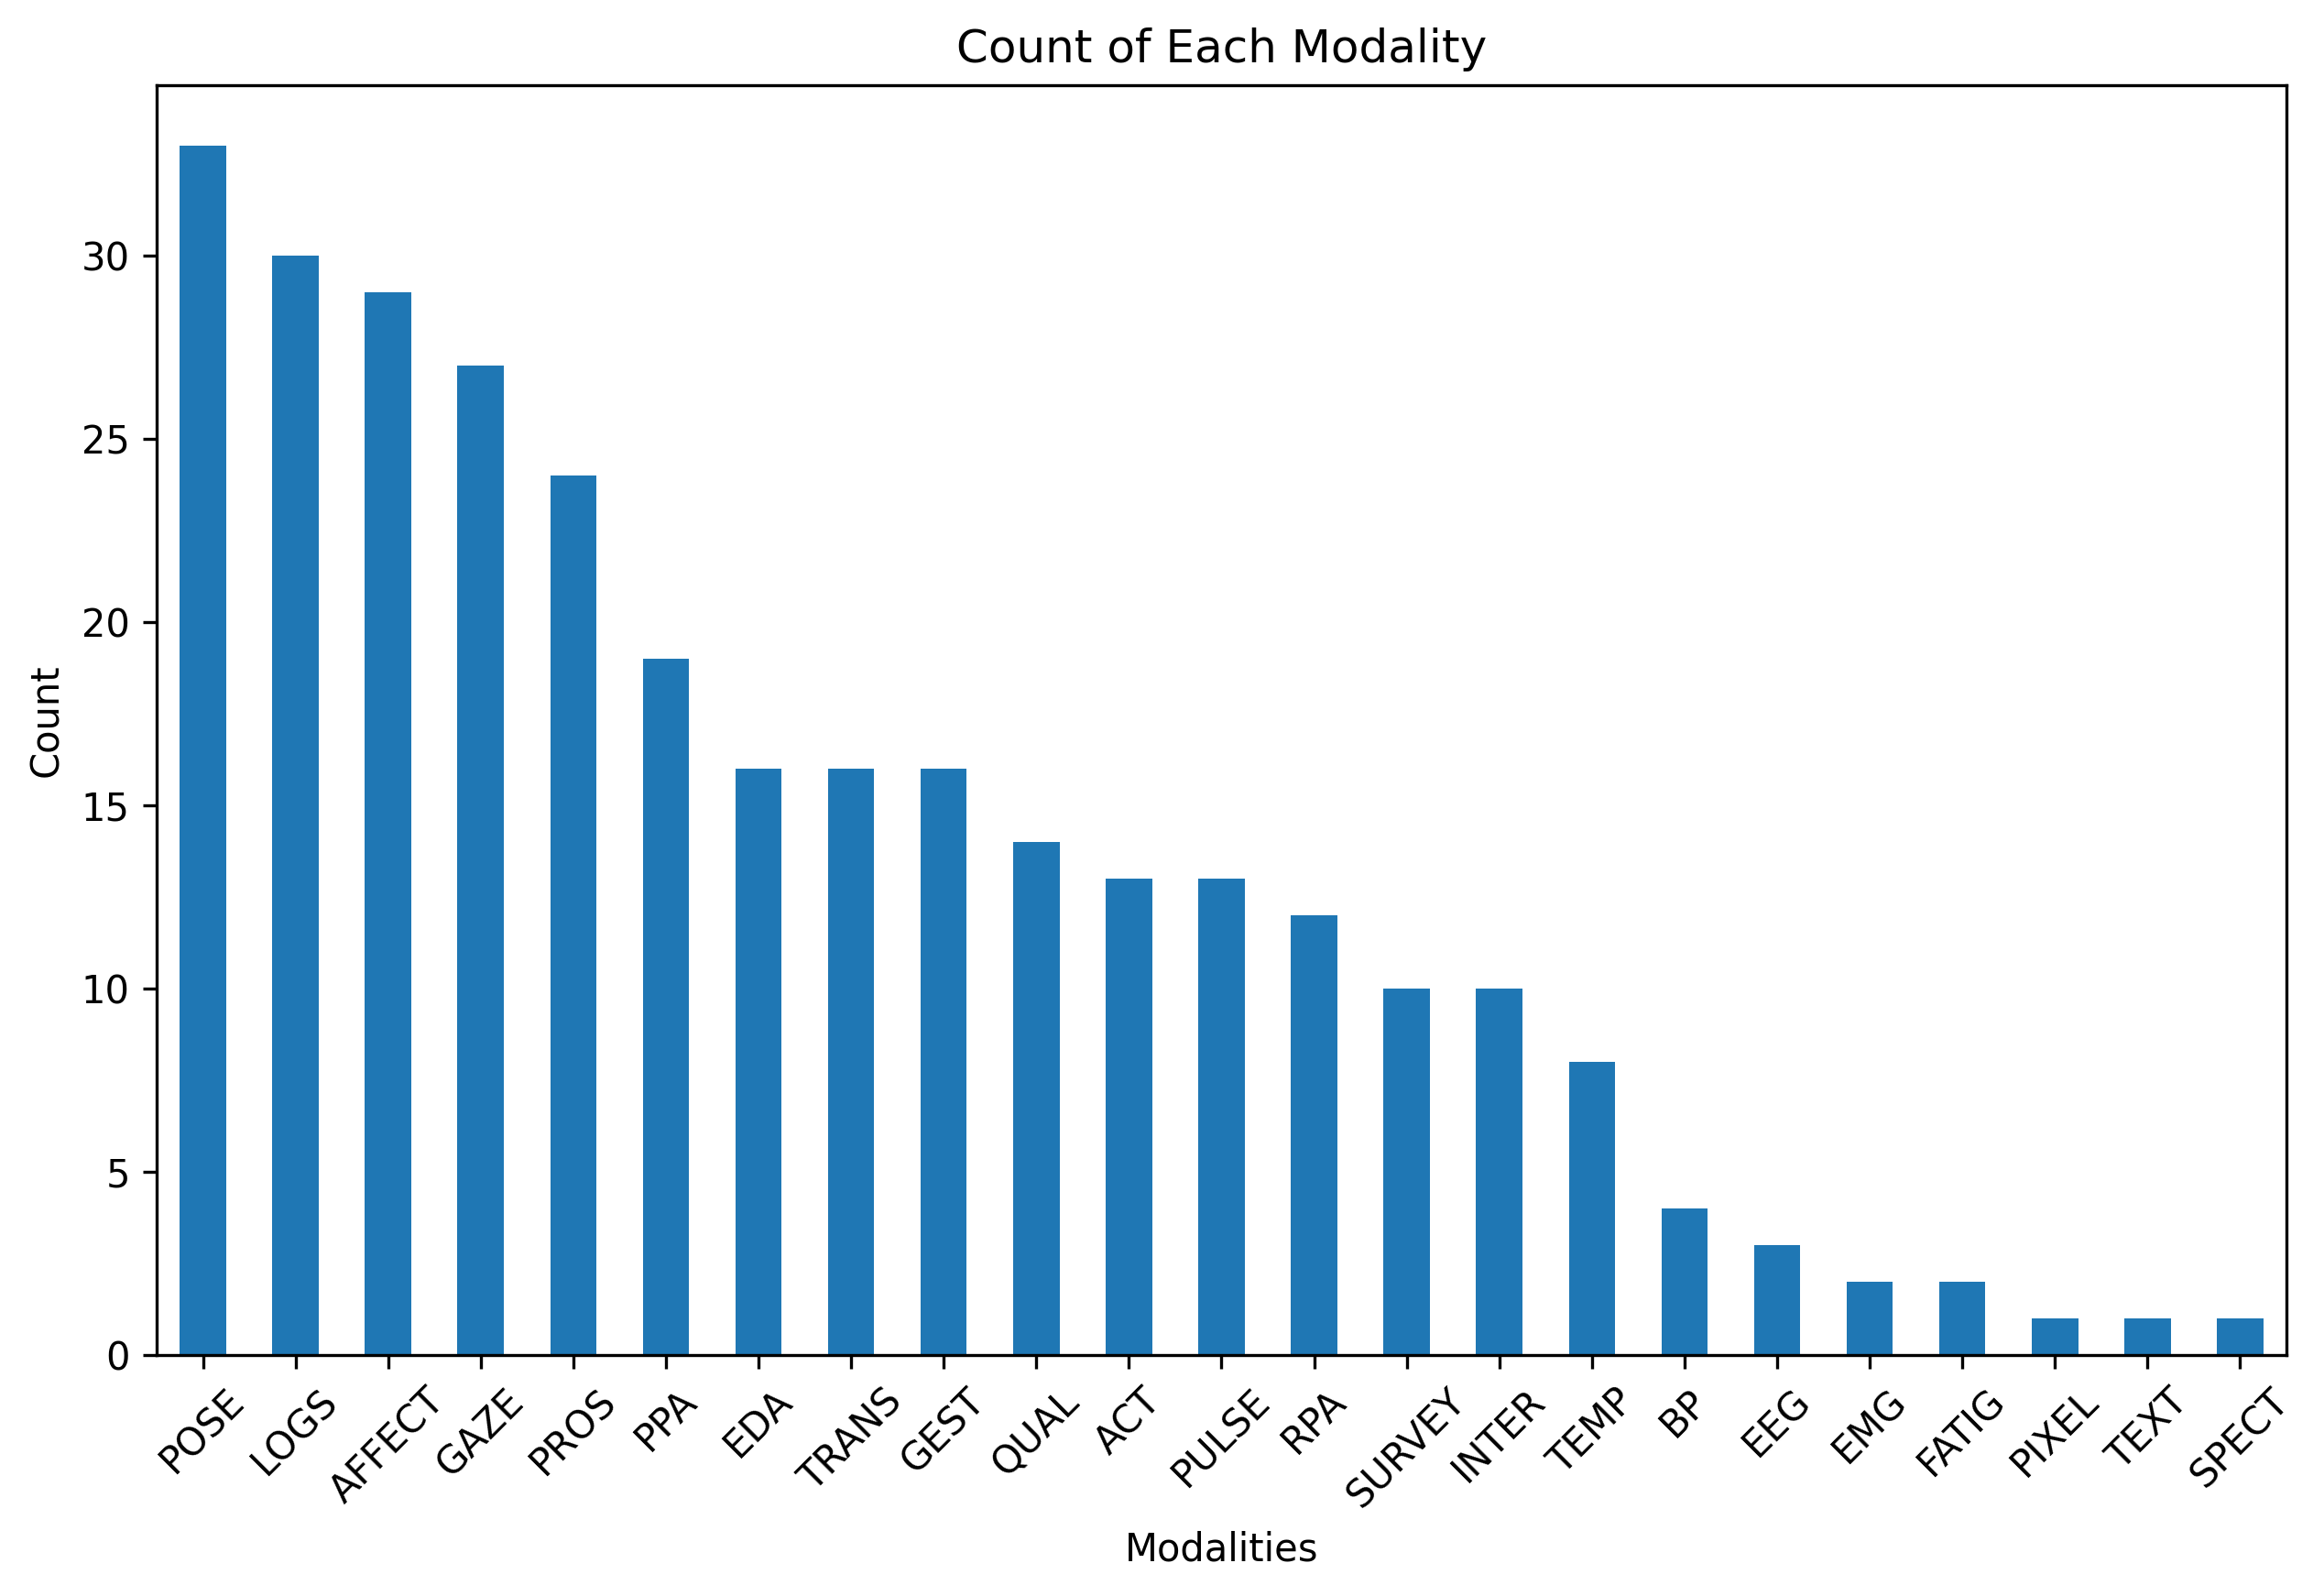
\includegraphics[width=\textwidth]{img/statistical_imgs/modalities.png}
        
        % Add footnote about the 1 paper with only 1 modality having multiple data collection mediums, so we consider it multimodal by our definition.
        
        \caption{Image 2}
    \end{subfigure}
    \hfill
    \begin{subfigure}[b]{0.45\textwidth}
        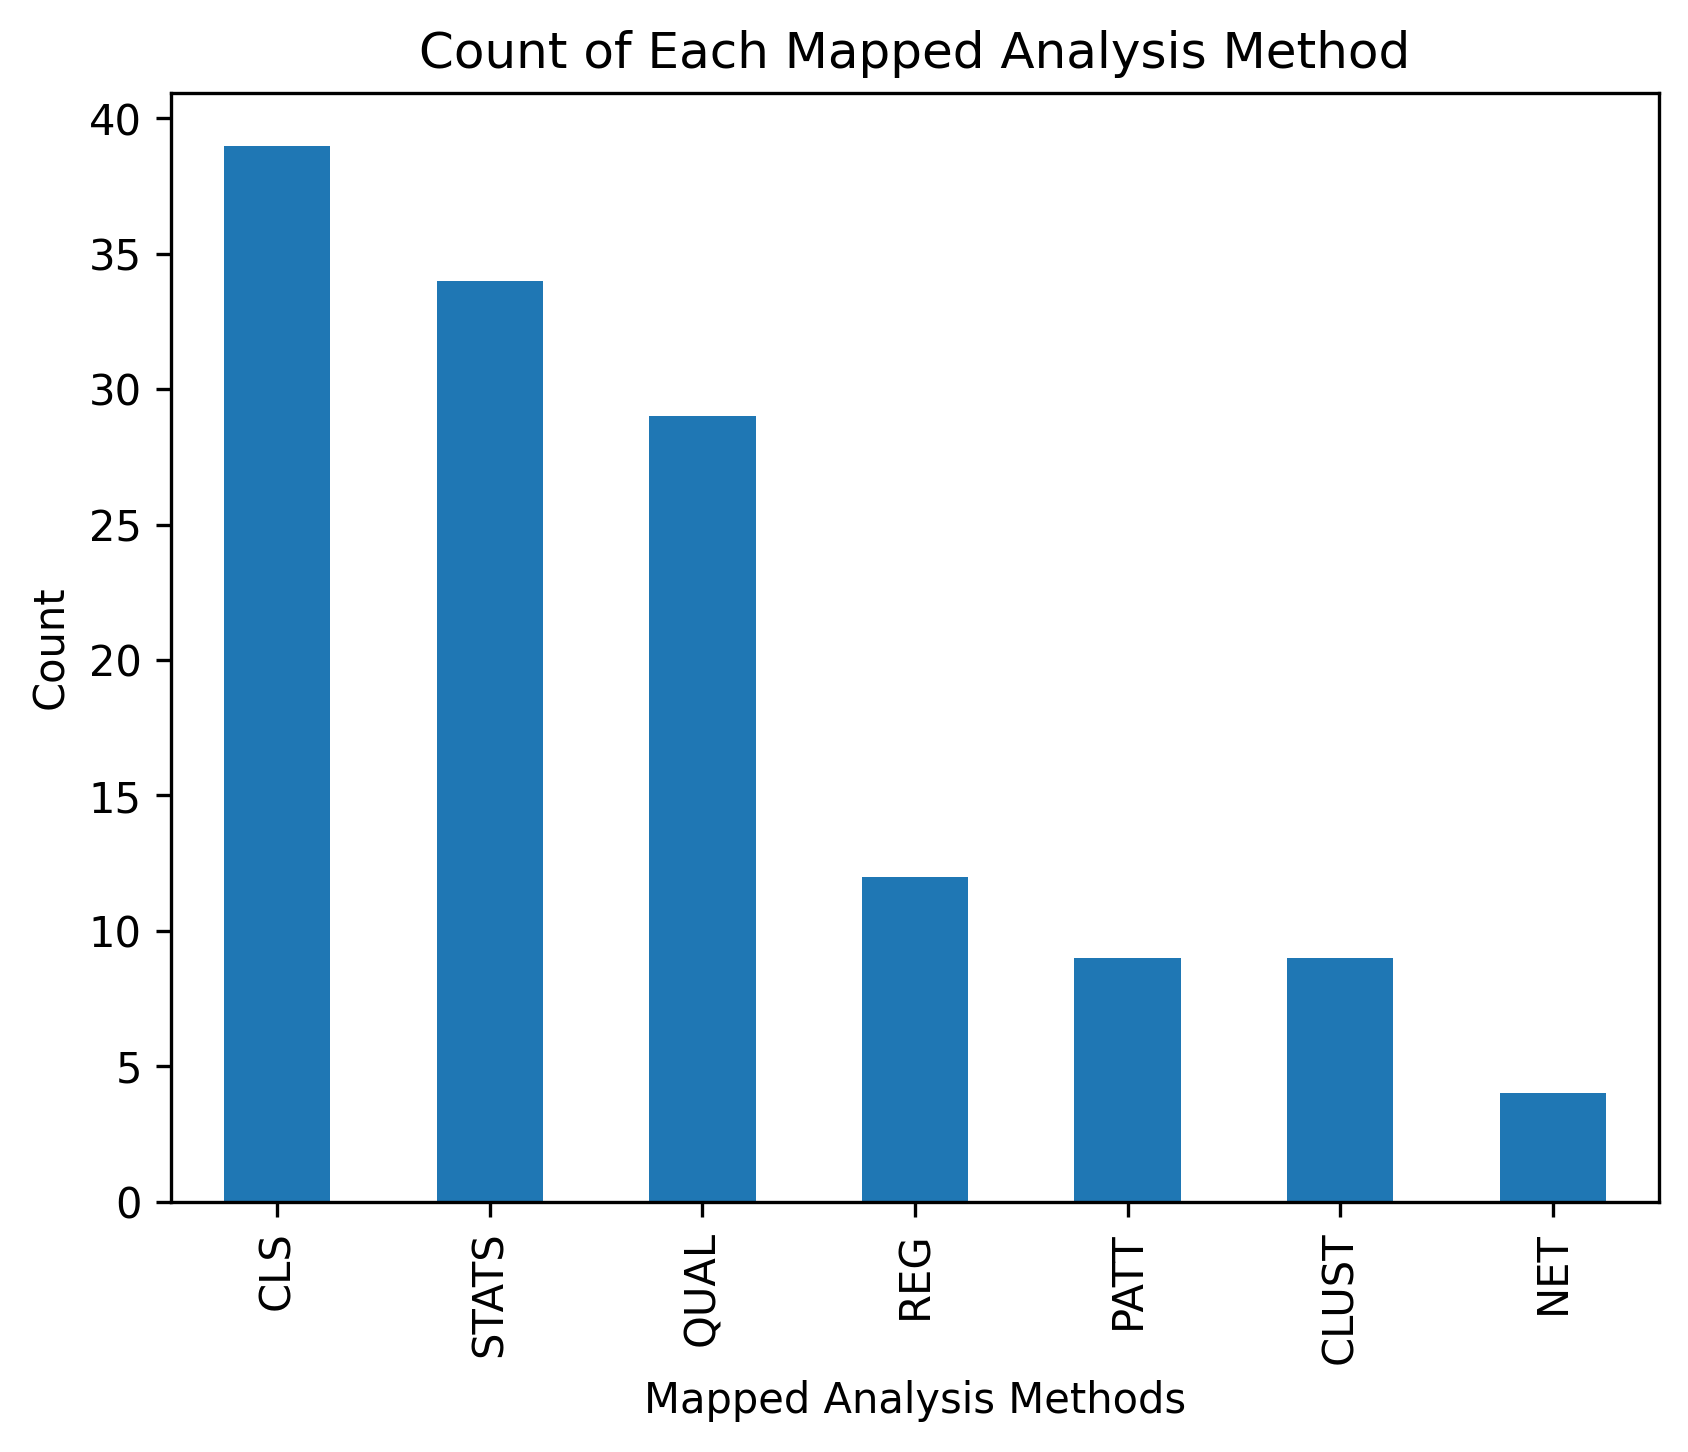
\includegraphics[width=\textwidth]{img/statistical_imgs/analysis_type.png}
        \caption{Image 3}
    \end{subfigure}
    \hfill
    \begin{subfigure}[b]{0.45\textwidth}
        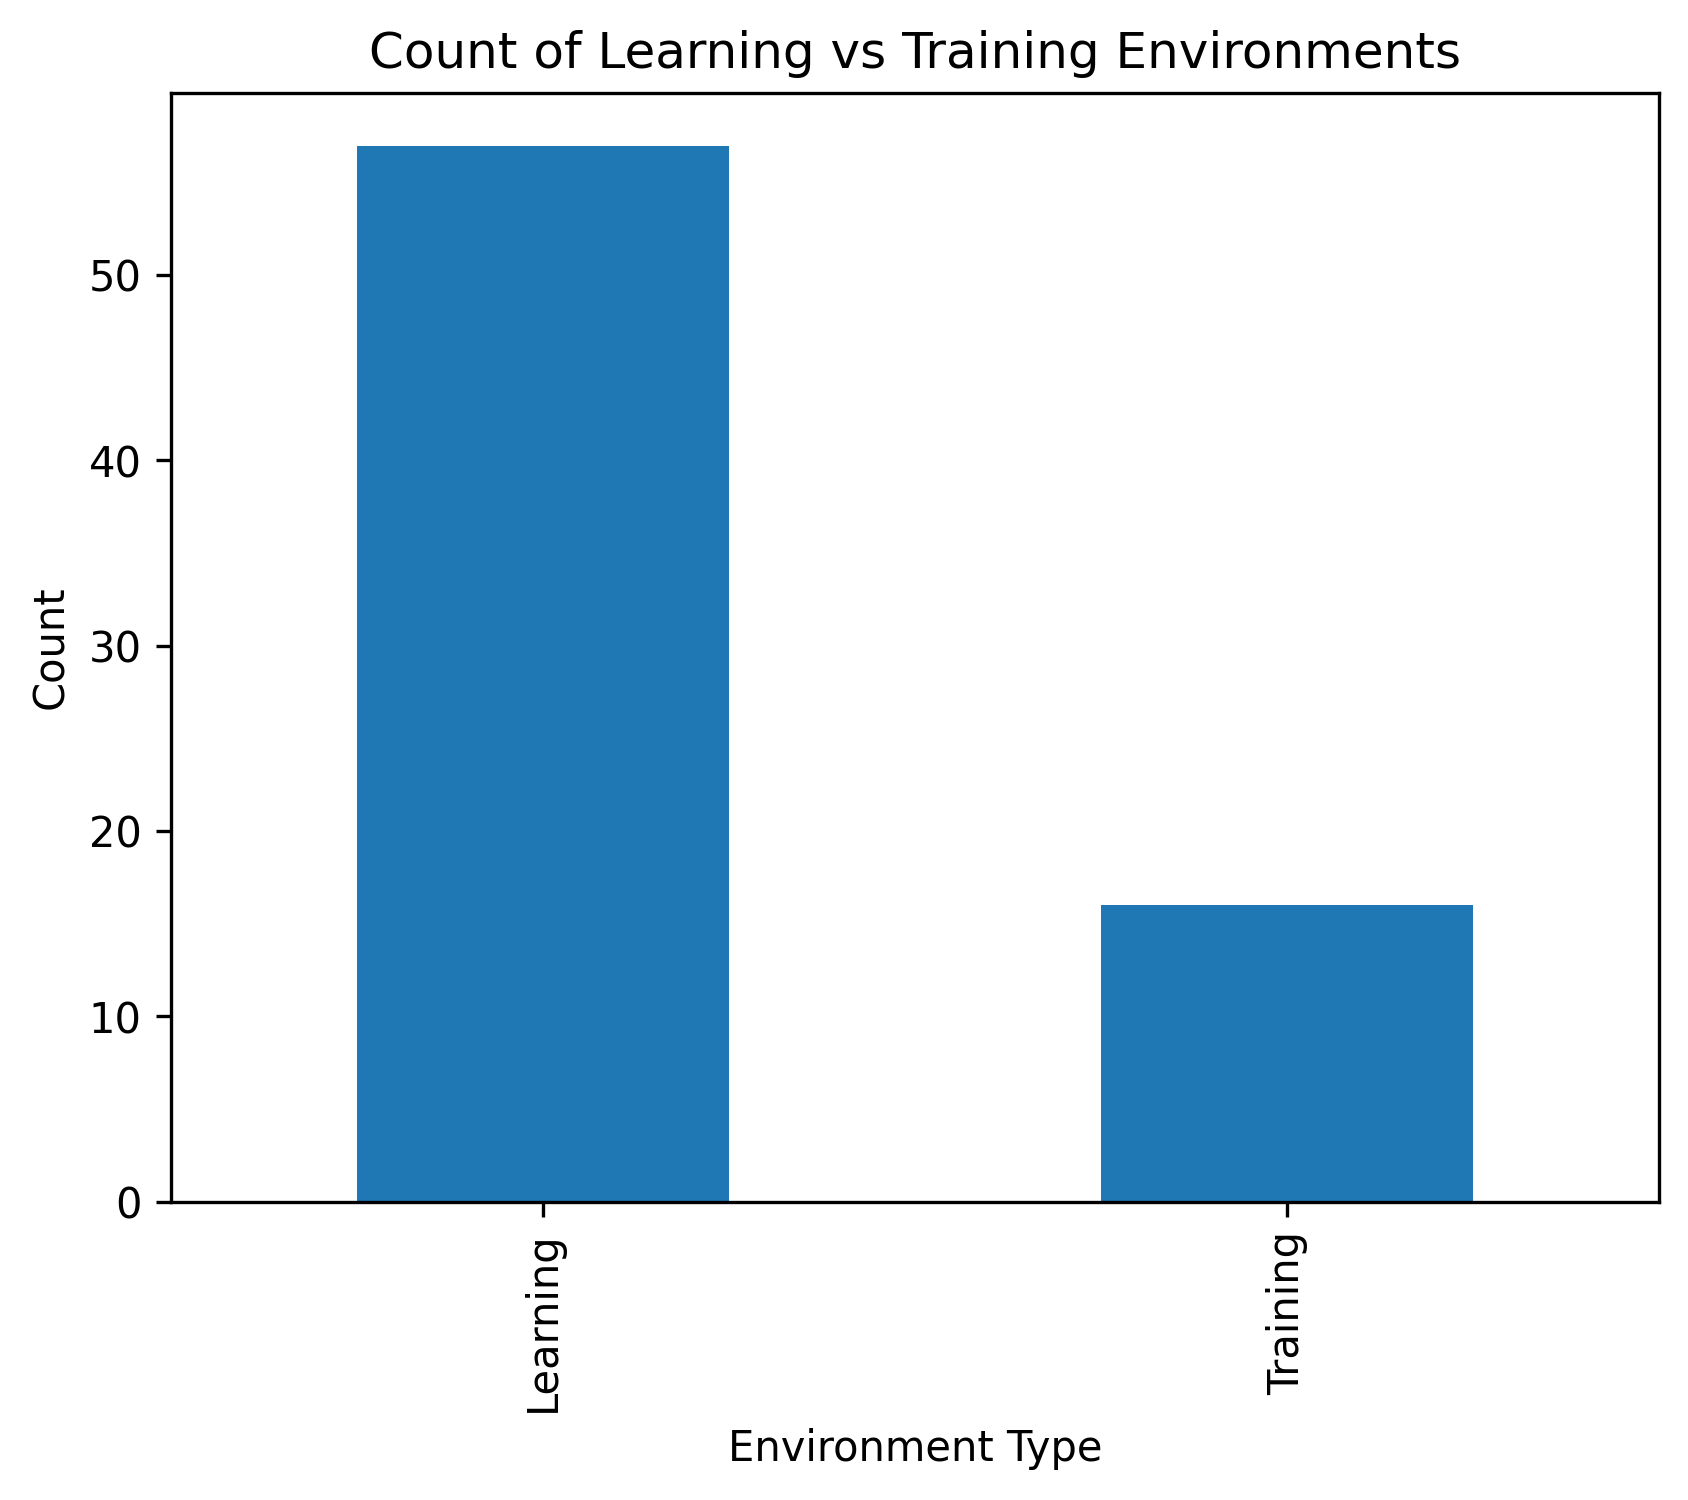
\includegraphics[width=\textwidth]{img/statistical_imgs/learning_vs_training_envs.png}
        \caption{Image 4}
    \end{subfigure}
    \begin{subfigure}[b]{0.33\textwidth}
        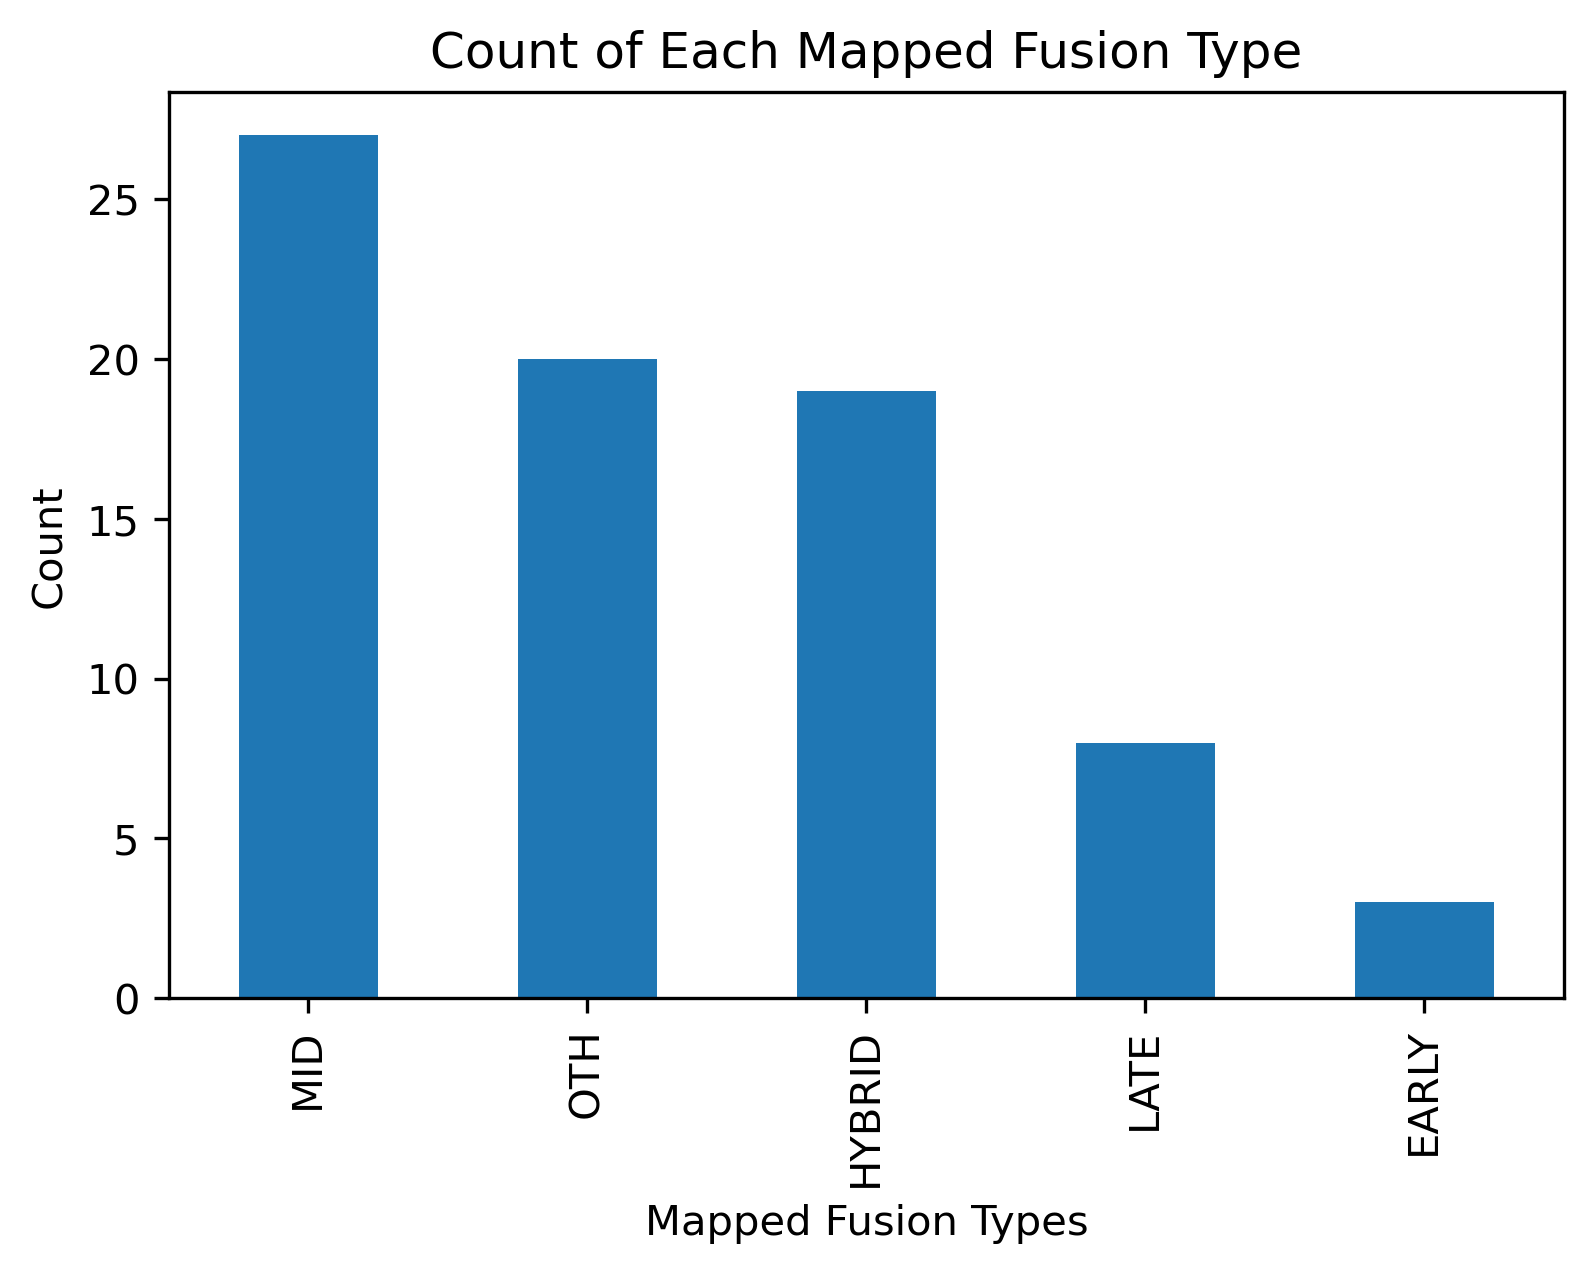
\includegraphics[width=\textwidth]{img/statistical_imgs/fusion_type with OTH.png}
        \caption{Image 5}
    \end{subfigure}
    \\
    \begin{subfigure}[b]{0.33\textwidth}
        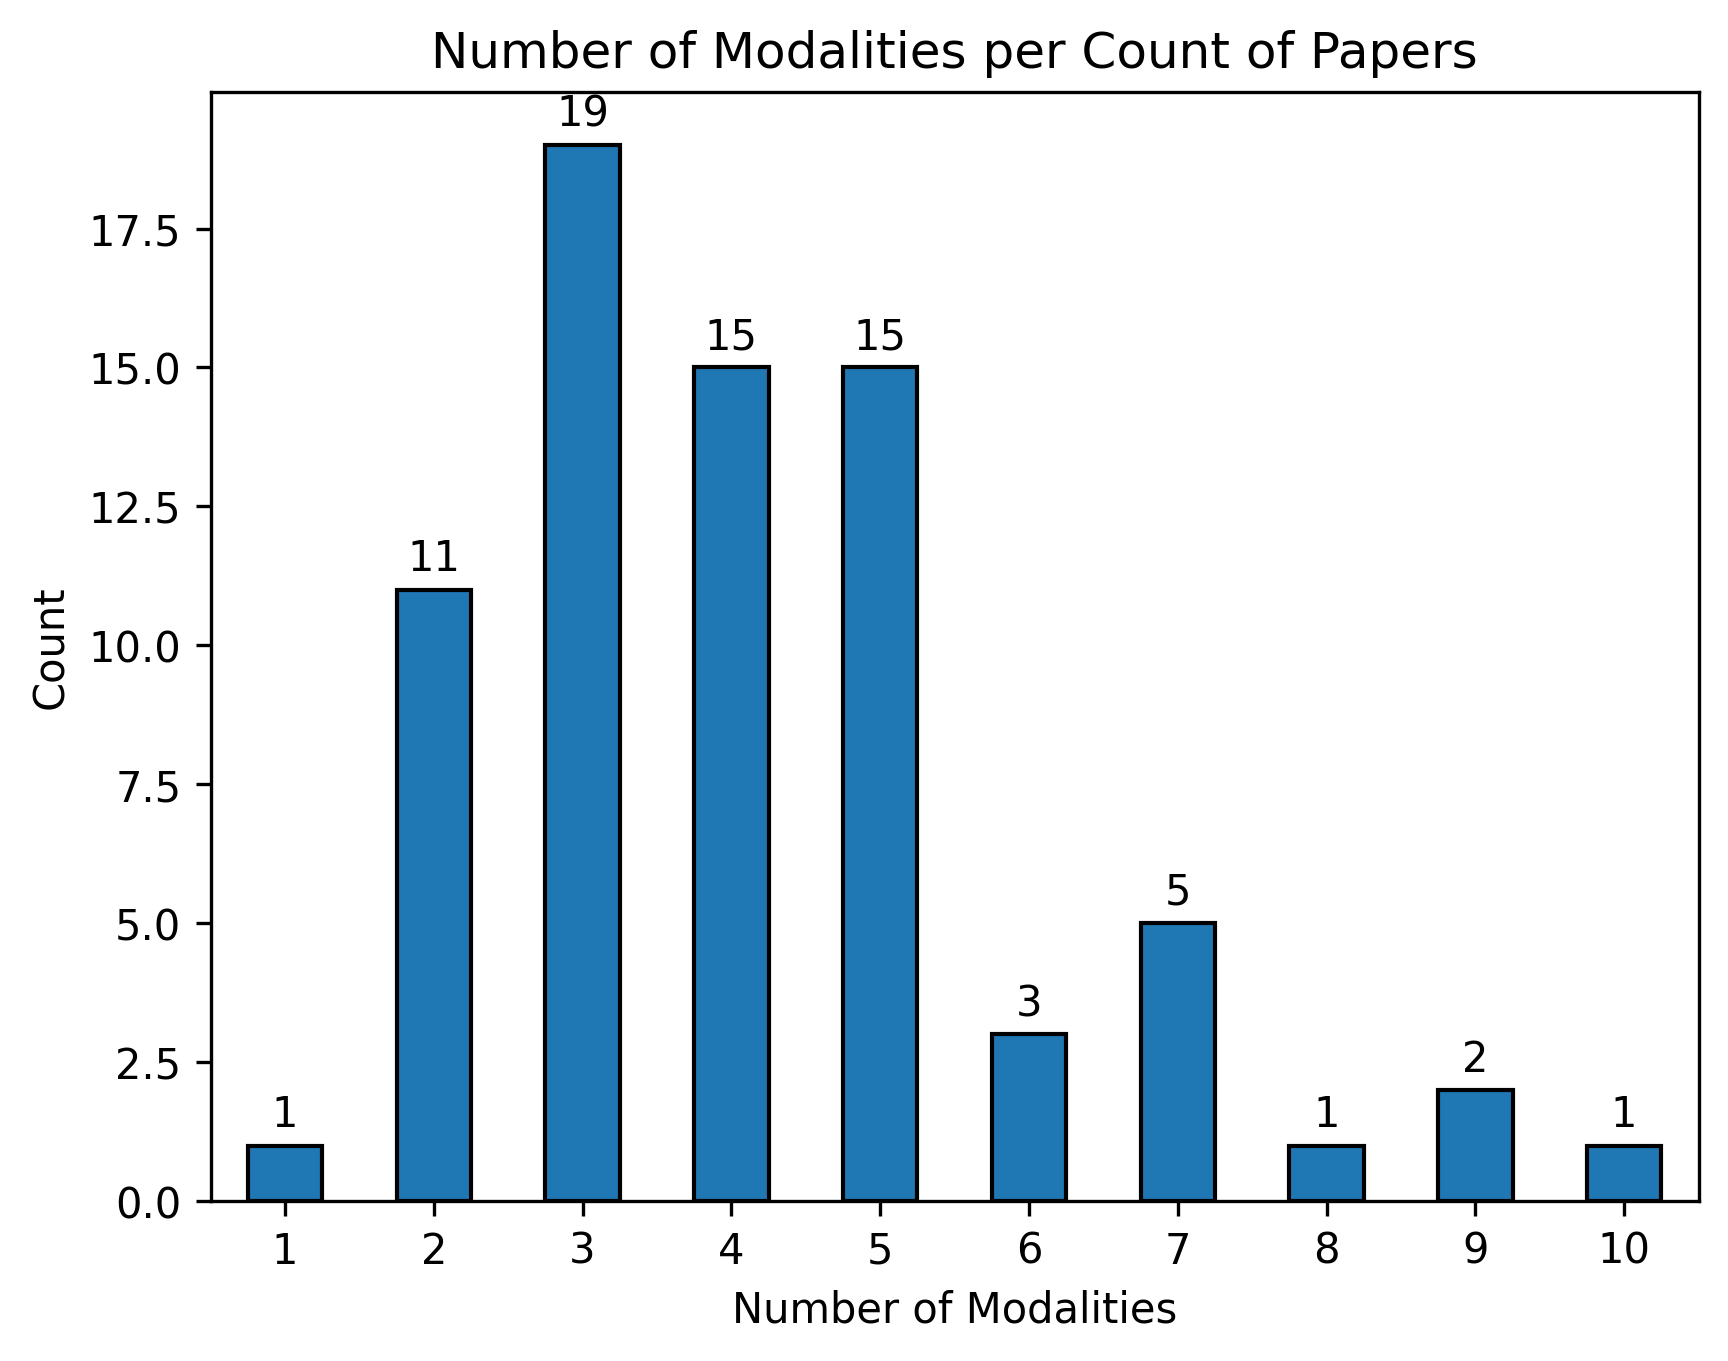
\includegraphics[width=\textwidth]{img/statistical_imgs/number of modalities per count of papers.png}
        \caption{Image 6}
    \end{subfigure}
    \hfill
    \begin{subfigure}[b]{0.33\textwidth}
        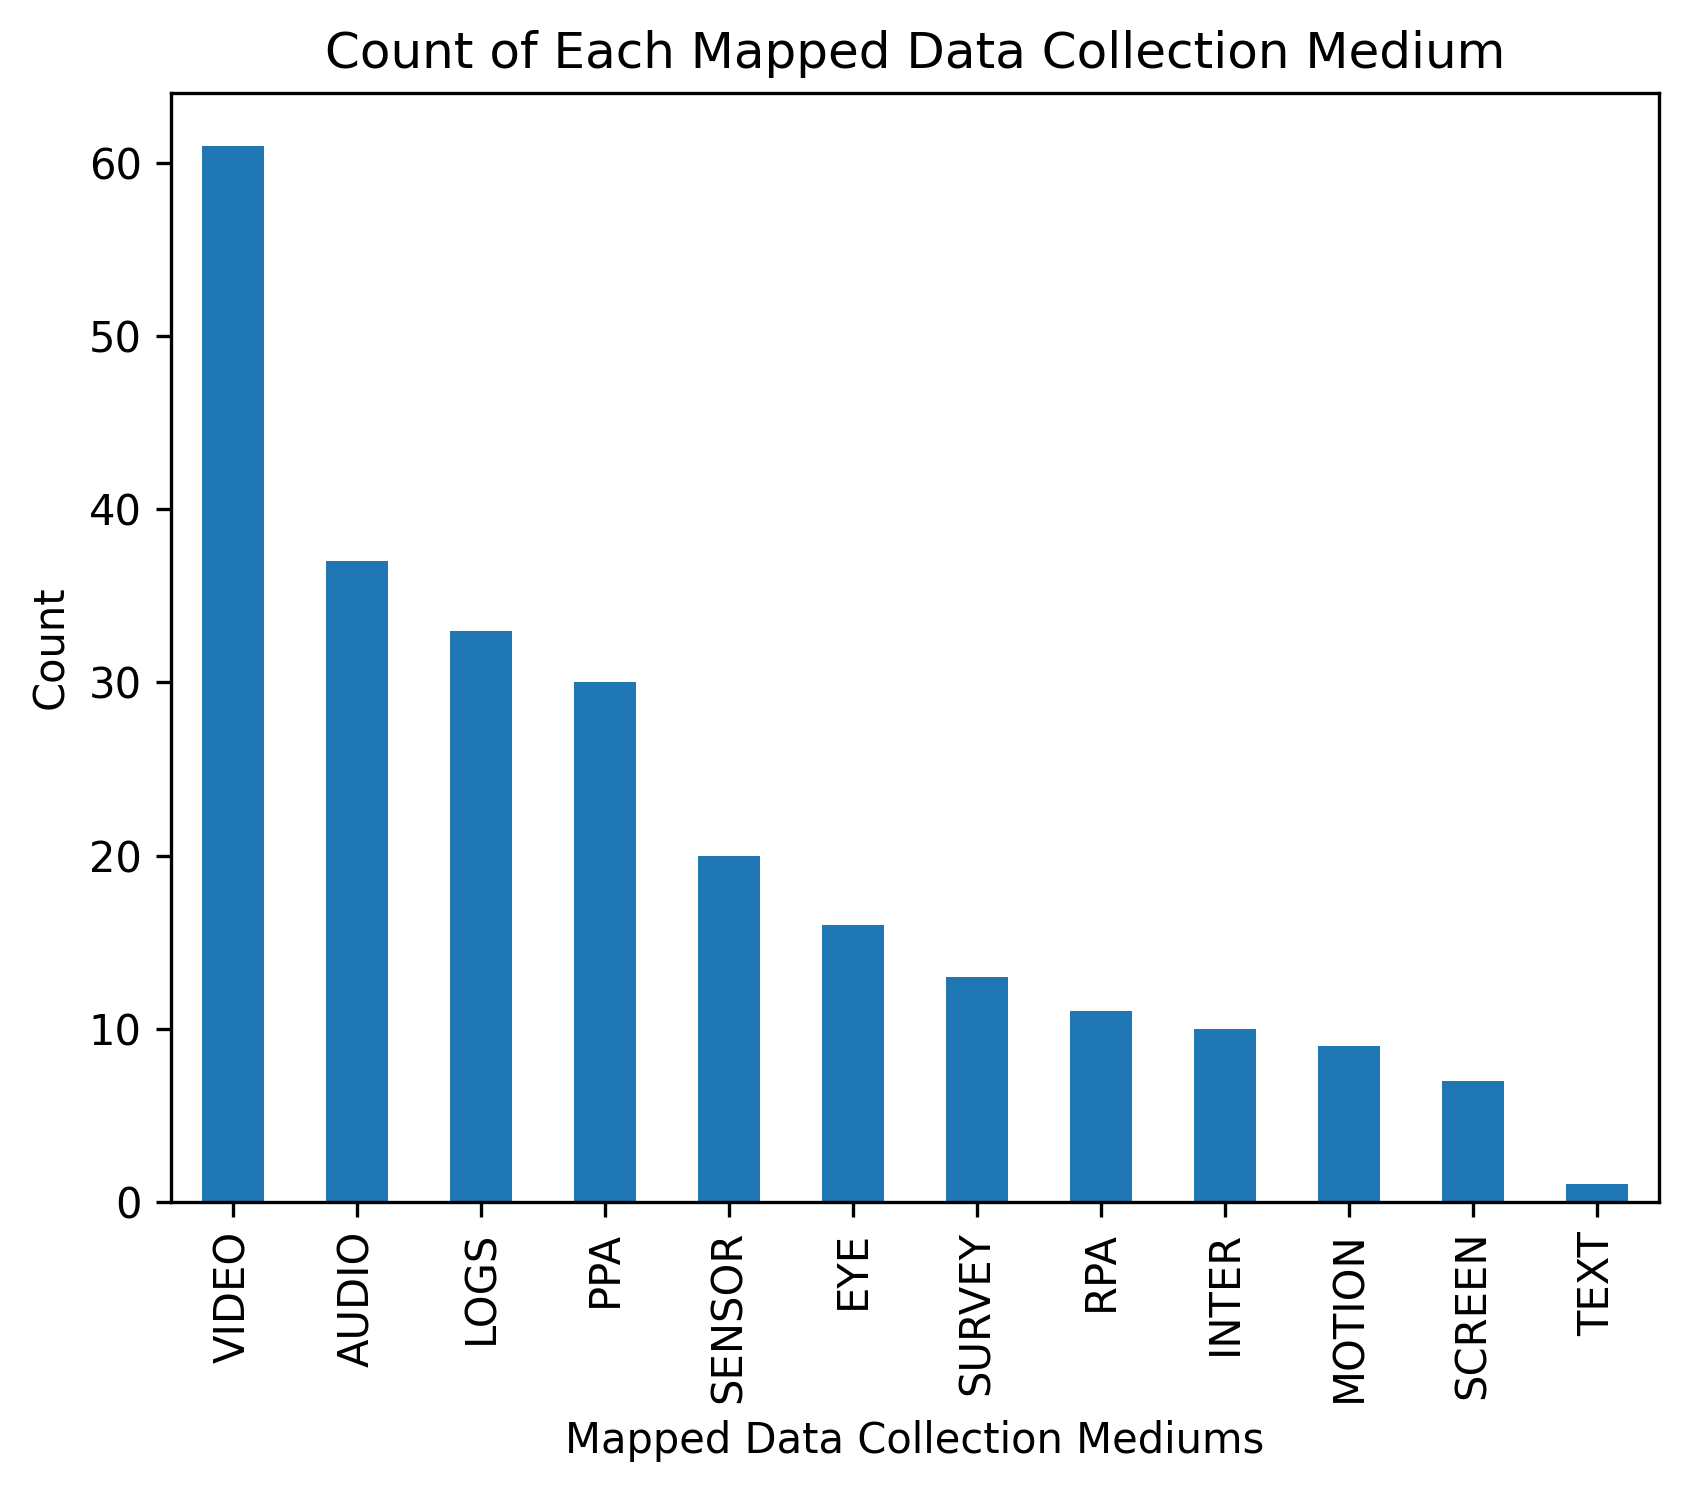
\includegraphics[width=\textwidth]{img/statistical_imgs/data_collection_mediums.png}
        \caption{Image 7}
    \end{subfigure}
    \\
    \begin{subfigure}[b]{\textwidth}
        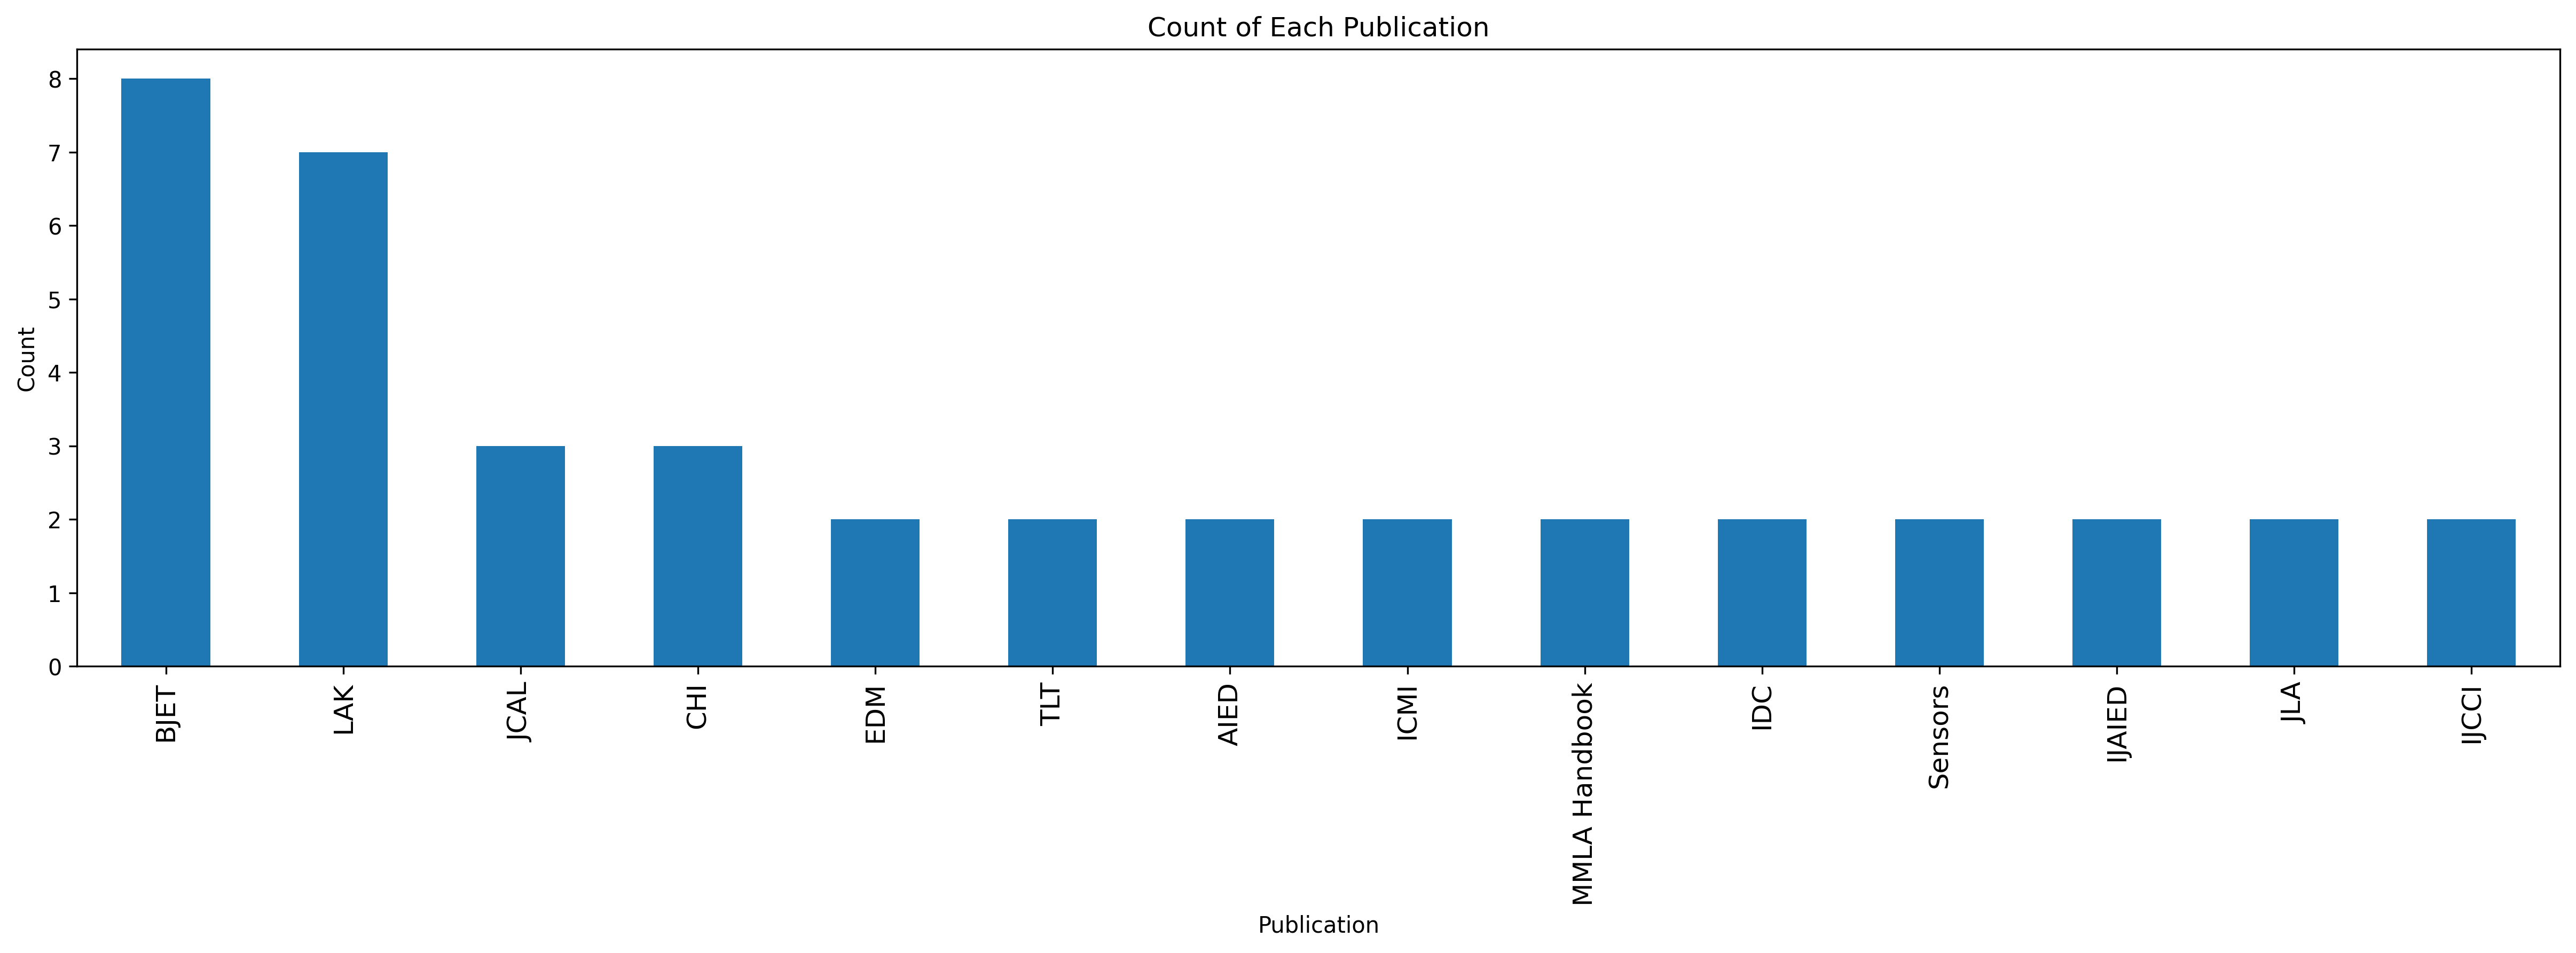
\includegraphics[width=0.8\textwidth]{img/statistical_imgs/publications_w_o_others.png}
        \caption{Large Image}
    \end{subfigure}
    \caption{Composite figure with 7 small images and 1 large image}
\end{figure}


\section{Discussion} \label{sec:discussion}
% Recap what we have done and findings

% Comprehensive review of research methods applied to multimodal learning and training environments
% A novel citation graph method for corpus reduction
% Qualitative analysis of current body of literature (subdomains + aggregate)
% Also discuss implications, limitations, and future research directions with MMLA
% Address Need for mid fusion

% Discuss (overall, in the aggregate):
    % Results
    % SOTA
    % Challenges
        % -"One of the biggest challenges in multimodal learning analytics is that the large volume of rich, multimodal data collected requires significant human time and effort to make sense of."
        % -"Making sense of all the richness that exists in multimodal data can be highly time-consuming."
        % -"Data from different sources are often difficult to integrate."
        % -"In practice, however, the increased complexity resulting from the additional collection of multimodal data presents unique challenges"
        % Codesign, explainability, trust (challenge/gap as a whole for the field).
        % Overall challenge: class size/data. Majority of methods used to analyze case studies or classroom-sized study participants. This is not a lot of data and may help explain why DL methods are not as common as you would expect.
            % limited amount of data available to properly train
                % -"data is limited, which represents one of the major challenges for building robust and reliable multimodal models"
                % -"training a model on a reduced dataset introduces a bias to the model, affecting the validity of the model’s predictions when the data inputs come from a different distribution than the training set. "
            % small set of students (overall challenge)
            % Small, imbalanced datasets (cite CSEDU, AIED, AIED2)
            % lack of representative data in open datasets (i.e., few focusing on children/education) (overall challenge)
            % Generalizability:
                % Finally, the design and sample size of the focus group do not allow us to generalize the results. 
                % The limited number of pair work EEs does not allow us to make any strong claims in terms of the framework’s reliability. 
        % Explainability: making sense of the data (overall challenge)
        % Subjectivity: the uncertainty arising from the [subjective] annotations may influence the resulting model structures, parameters and interpretation. I.e., tough to generalize (overall challenge)
        %   Cite: C&E, IUI, EAAI
        % Diversity:
        %  "...the subject pool is not overly diverse, limiting our ability to explore culture or ethics-related factors in the model reliably"
        % "Obtaining and labelling data is indeed a costly process especially in the context of education"
        % 
    % Research gaps
    %   Domain specificity and lack of generalizable approaches
    %   Small/imbalanced/unrepresentative data (need large open sets)
    %   Multimodal, conversational agents
    %   Lack of longitudinal work
    %   XAI
    
\subsection{Implications}

% Publications: BJET and LAK most popular journal/conference for applied MMLA and quantitative analysis
% Learning more popular than training currently
% Video, audio, logs, ppa most popular mediums
% Pose, logs, affect, gaze, and prosodic speech appear to be the most popular modalities.
% Most multimodal work considers 2-5 modalities per paper (cite figure if necessary, but shouldn't be needed. Can just use raw counts)
% Classification, stats, qual most popular analysis methods
% Mid fusion and hybrid fusion most popular
% Not necessary to do tons of modalitites, but focus on a few that are the most informative
% Should consider data fusion to inform environment, particularly mid fusion by fusing observable, derived features

\subsection{Limitations}
The major limitations of this work involve the use of Google Scholar to conduct the literature search and the use of a citation graph for programmatic corpus reduction. Both are discussed in the following paragraphs.

\subsubsection{Google Scholar.} While Google Scholar is widely used by researchers across both academia and industry, it poses a challenge for reproducibility. Like Google Search, Google Scholar is a non-deterministic, proprietary search algorithm. Factors such as the individual user conducting the search, the user's geolocation, the date the search was conducted, and the user's search history may all affect how Google Scholar collates search results. Google may also perform A/B testing in live environments to determine which version of its algorithm users deem more effective. The algorithm is also (presumably) continually evolving, and users are unable to know exactly which version of the algorithm is used to conduct a particular search. As such, there is little expectation that our initial corpus will be able to be reconstructed \textit{in its exact form} without at least some degree of variability.

The authors are confident the degree of variability from different Google Scholar searches does not prohibit the \textit{overall} reproducibility of the initial corpus. While SerpAPI's web scrape method is proprietary, the creators address several of our concerns in their documentation\footnote{https://serpapi.com/}. The API's search does not use information from any individual user's Google account when conducting the web scrape, as no Google account is attached to the SerpAPI account, API key, or API calls themselves. Instead, calls are made via proxy and random headers, as illustrated in Figure \ref{fig:serpAPI}. When trying to reproduce the API's results via manual search, SerpAPI recommends using the URL in the API's JSON results in ``incognito mode". 

\begin{figure}
    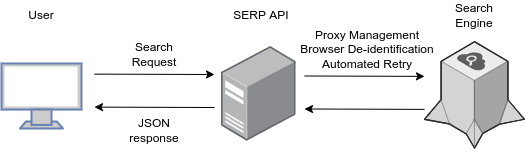
\includegraphics[width=\textwidth]{img/SERP_API_diagram.drawio.png}
    \caption{Searching Google Scholar via SerpAPI.}
    \label{fig:serpAPI}
\end{figure}

Additionally, we reached out to SerpAPI directly and asked, ``Does SerpAPI attach personal or identifying information when making request?", to which SerpAPI responded, ``No, we don't add any personal information." SerpAPI also stated, ``...others can reproduce your results by using Google Scholar website, if they use the same search criteria...", but we believe this to be an overstatement given Google's lack of transparency with regard to exactly which algorithm is being used in any single search. While we cannot guarantee perfect reproducibility due to the aforementioned issues, we can state with a reasonable degree of confidence that our own individual search biases did not influence the initial search results (outside of the choosing of the search terms) due to how SerpAPI handles API calls to Google Scholar. For reference, this review's literature search was conducted by an author of this paper in Nashville, TN, USA on October 22, 2022.

\subsubsection{Citation graph pruning.} 

As discussed in Section \ref{subsec:study_selection}, we initially pruned our corpus using quantitative means via the use of a citation graph. In doing this, it is possible we excluded relevant works from our corpus based on them only having cited or been cited by a minimal number of other works in our corpus. This literature review is a survey of the prominent methods, practices, and approaches researchers are applying to multimodal learning and training environments. As such, the authors agreed that if a work did not utilize a large degree of previous research (i.e. cite several other works in the corpus) or serve as a base from which a large degree of other researchers have built upon (i.e. be cited by several other works in the corpus), then that work was likely outside the scope of our review. Considering our corpus was still largely comprised (over 50\%) of works later deemed to be outside the scope of this review after graph-based pruning, the authors are confident that few papers directly pertaining to multimodal learning and training environments were discarded as a result of graph-based pruning.

\subsection{Other Limitations}.
% Limitation for one paper not peer reviewed, but this is okay because all papers accepted somewhere and therefore refereed to some degree. 

% Search term limitation add
%   we only searched "multimodal," so MMLA research done without using this word may not be included in our initial search

% ChatGPT not included (came out right after our literature search.)

\subsubsection{Future Research Directions} 
% Additional modalities
% Text with LLMs (search ended a month prior to ChatGPT release)
% Textless NLP 
% Domain-specific directions
% Infrastructure
% ChimeraPy
% Further automating corpus reduction process

\section*{Conflict of Interest Statement}

\section*{Author Contributions}

\section*{Funding}
% All grants involved

\section*{Acknowledgments}

%%
%% The next two lines define the bibliography style to be used, and
%% the bibliography file.
\bibliographystyle{ACM-Reference-Format}
\bibliography{references, zotero_references, corpus_papers, uuid_references}

%%
%% If your work has an appendix, this is the place to put it.
% \appendix

\end{document}
\endinput
%%
%% End of file `sample-manuscript.tex'.